\documentclass{beamer}
\usepackage[en]{zafu}
\usepackage[utf8]{vietnam}
\usepackage{ragged2e}
\usepackage{movie15}
\usepackage{listings}
\usepackage{xcolor}
\usepackage{multicol}


\definecolor{codegreen}{rgb}{0,0.6,0}
\definecolor{codegray}{rgb}{0.5,0.5,0.5}
\definecolor{codepurple}{rgb}{0.58,0,0.82}
\definecolor{backcolour}{rgb}{0.95,0.95,0.92}

\lstdefinestyle{mystyle}{
	backgroundcolor=\color{backcolour},   
	commentstyle=\color{codegreen},
	keywordstyle=\color{magenta},
	numberstyle=\tiny\color{codegray},
	stringstyle=\color{codepurple},
	basicstyle=\footnotesize,
	breakatwhitespace=false,         
	breaklines=true,                 
	captionpos=b,                    
	keepspaces=true,                 
	numbers=left,                    
	numbersep=5pt,                  
	showspaces=false,                
	showstringspaces=false,
	showtabs=false,                  
	tabsize=2
}

% \usepackage{xeCJK}

\setbeamerfont{normal text}{size=\small}

\definecolor{hrefcol}{RGB}{0, 0, 255}

% meta-data
\title{Backpropagation in Convolutional \\Neural Networks}
\subtitle{University of Information Technology}
\author{Nguyễn Đặng Đức Mạnh}
\date{\textit{a sand soldier of 3ker}}

% document body
\begin{document}

    \maketitle
	
    \section{Introduction}
    
    \begin{frame}
    	\frametitle{Geoffey Hinton}
    	
    	\begin{columns}
    		\column{0.5\textwidth}
    		\centering
    		\justify
    		Professor Geoffrey Hinton, the Nobel Prize winner in Physics in 2024, is also the one who popularized the backpropagation algorithm, which is the foundation for the remarkable development of AI
    		
    		\column{0.5\textwidth}
    		\begin{flushright}
    			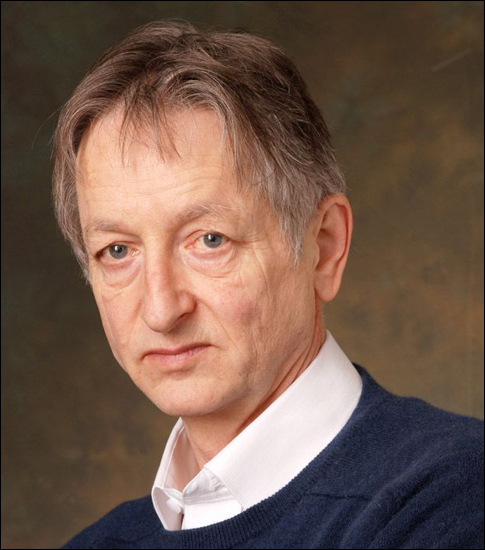
\includegraphics[width=0.8\textwidth]{src/hinton}
    		\end{flushright}
    	\end{columns}
    \end{frame}
    
    \begin{frame}
    	\frametitle{Backpropagation algorithm}
    	\justify 
    	For a model \( m_{\theta} \) parameterized by the parameter set \( \theta \), backpropagation is an algorithm that automatically updates the parameters \( \theta \) to optimize \( m_{\theta} \) based on the rules of derivatives..
% TODO: \usepackage{graphicx} required
\begin{figure}
	\centering
	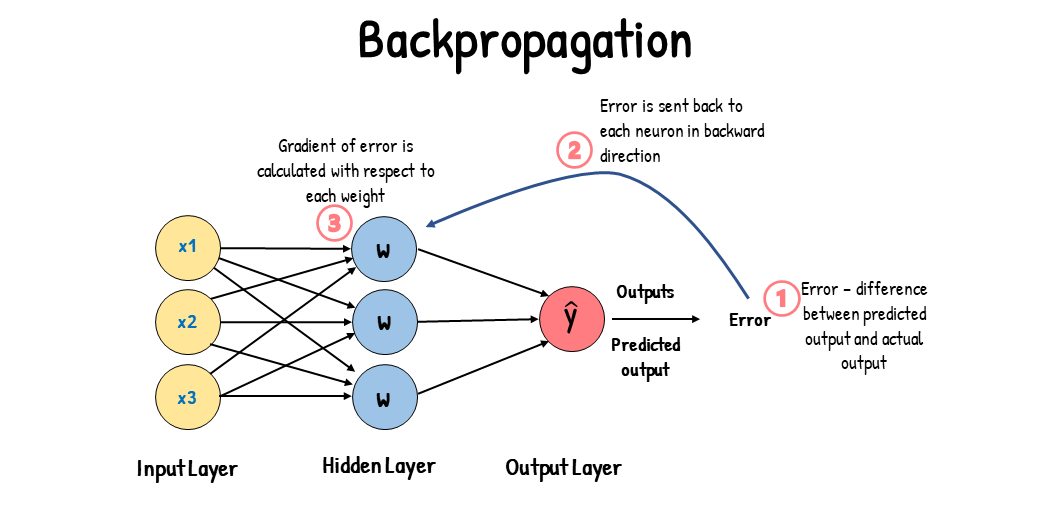
\includegraphics[width=0.8\linewidth]{src/18870backprop2}
	\label{fig:18870backprop2}
\end{figure}
    \end{frame}
    
    \begin{frame}
    	\frametitle{Convolution}
    	\justifying
    	The convolution operation has its origins in the field of signal processing. The kernel \( f \) acts as a signal detector; the more the signal \( g \) resembles \( f \), the greater the response (output). A well-known application of convolution can be seen in the Fourier Transform.
    	
% TODO: \usepackage{graphicx} required
\begin{figure}
	\centering
	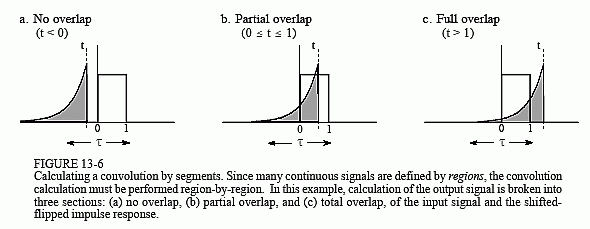
\includegraphics[width=0.7\linewidth]{src/sig_conv}
	\label{fig:sigconv}
\end{figure}
    \end{frame}
    
    
    \begin{frame}
    	\frametitle{Convolutional Neural Network}
    	\justifying 
    	The convolution operation was subsequently applied alongside the backpropagation algorithm in computer vision tasks and began to become the dominant method to this day. The Artificial Neural Networks that use convolution for feature extraction are called Convolutional Neural Networks (CNNs). 
    	 
    	\begin{figure}
    		\centering
    		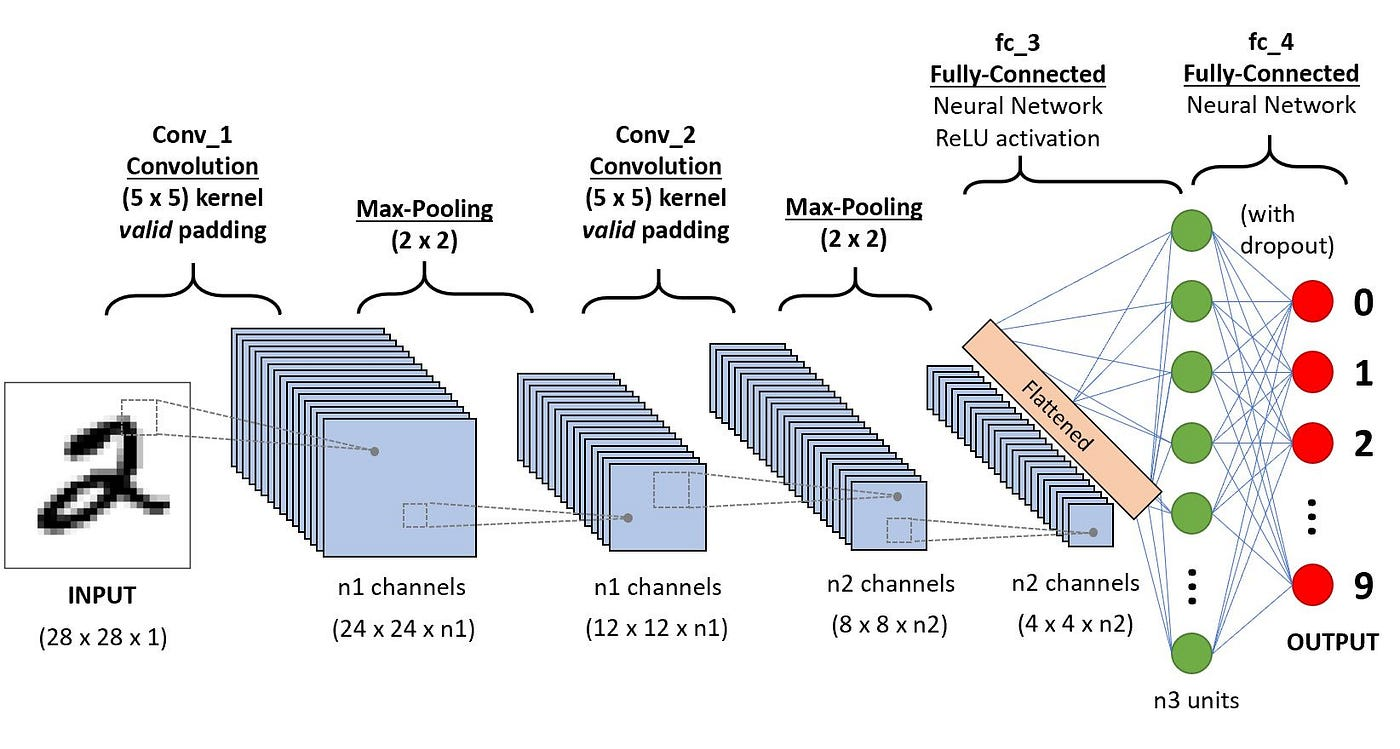
\includegraphics[width=0.7\linewidth]{src/conv_net}
    	\end{figure}
    \end{frame}
    
    
    \begin{frame}
    	\frametitle{Objective}
    	\begin{itemize}
    		\item Derive the formula for the convolution derivative.
    		\item Develop the backpropagation process.
    		\item Build and train a CNN based on the above theory.
    		\item Validate the theory with experimental results.
    	\end{itemize}
    \end{frame}
    
    
    \section{Theory}
    \subsection{Convolution}
    
    \begin{frame}
    	\frametitle{Misunderstanding}
    	\justifying
    	An RGB image has a shape of \([3, H, W]\), which means it is a 3-dimensional tensor. Similarly, a Conv2D operation has a kernel with 3 dimensions \([in\_channels, H_{conv}, W_{conv}]\), and there are \(out\_channels\) such kernels, rather than being 2-dimensional as shown in many illustrative documents.
    	
    	\begin{figure}
    		\centering
    		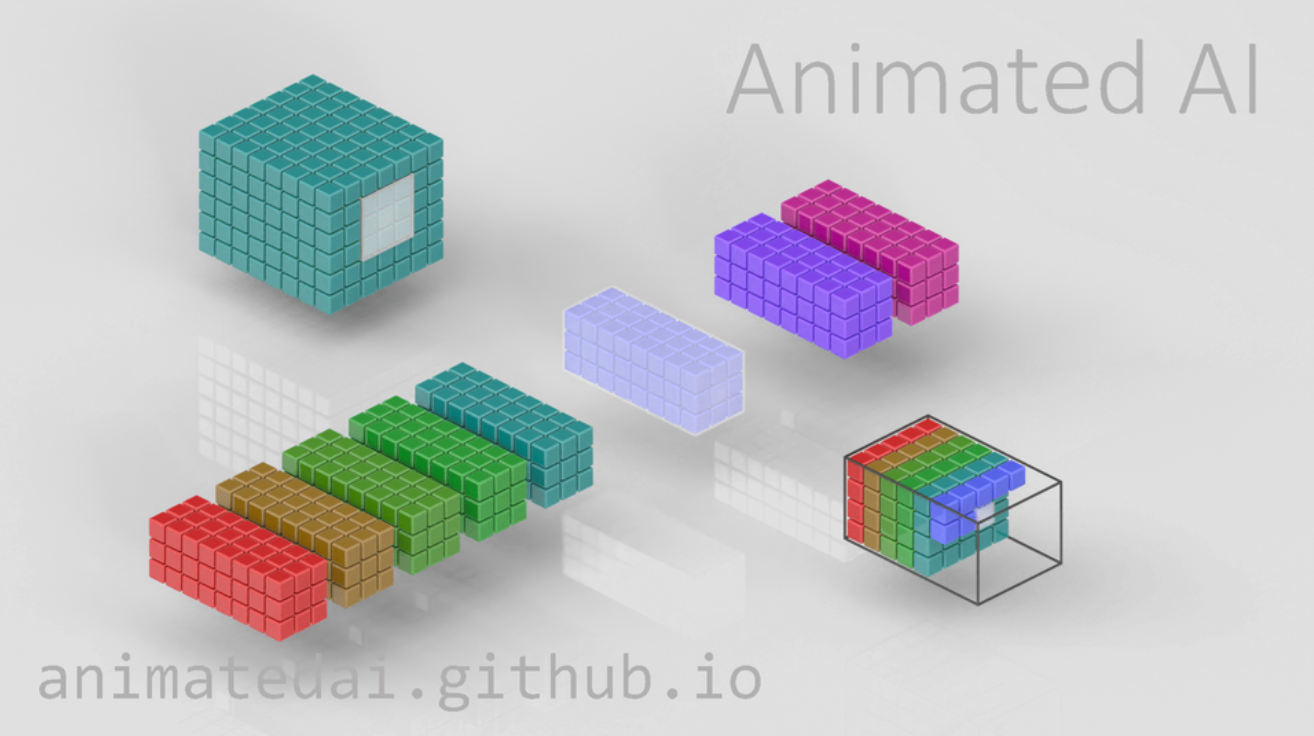
\includegraphics[width=0.7\linewidth]{src/true_conv}
    	\end{figure}
    \end{frame}
    
    \begin{frame}
    	\frametitle{Misunderstanding}
    	\justifying
    	However, the \(2D\) version is easier to explain, so in this slide, I will use \(2D\) matrices to represent the kernel and the input/output feature maps. However, please note that in reality, both the kernel and the feature maps are \(3D\) matrices (not counting the \(batch\_size\)). In the implementation, I will still use the \(3D\) version, which will be explained accordingly..
    	\begin{figure}
    		\centering
    		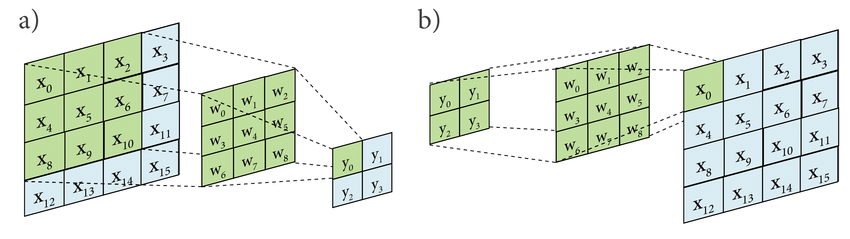
\includegraphics[width=0.7\linewidth]{src/conv2d}
    	\end{figure}
    \end{frame}
    
    \begin{frame}
    	\frametitle{Convolution}
    	\justifying
    	\tiny
    	In this slide, to avoid excessive explanations that may distract from the main focus, I would like to make the following assumptions:
    	
    	\begin{itemize}
    		\item The kernel and feature map are square matrices.
    		\item There is always a bias term.
    		\item \( \text{stride} = 1 \), \( \text{padding} = 1 \), \( \text{dilation} = 1 \), \( \text{groups} = 1 \).
    	\end{itemize}
    	
    	These assumptions may reduce generality, but they are very convenient for explaining and understanding convolution as well as its derivative. Once understood, generalizing is not difficult.
    	
    	\begin{figure}
    		\centering
    		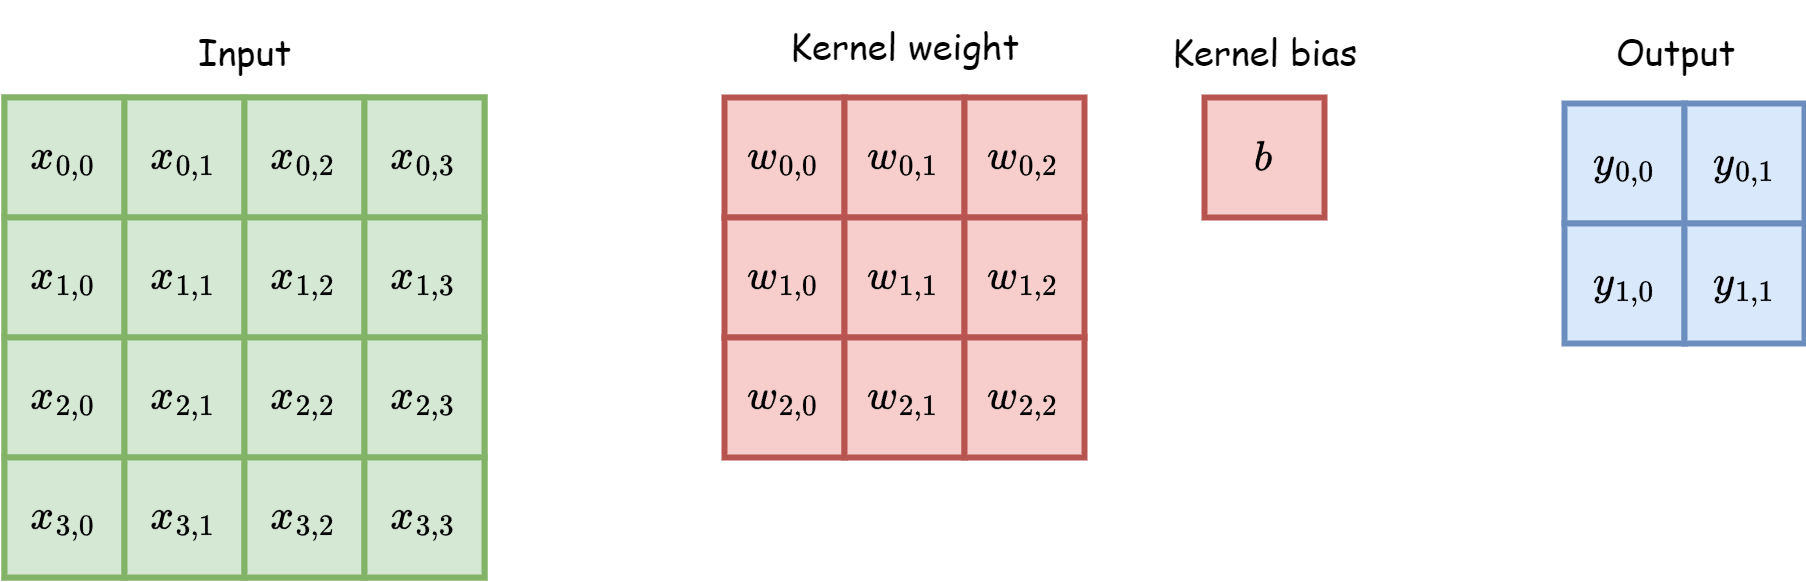
\includegraphics[width=0.8\linewidth]{src/conv.drawio (2).png}
    	\end{figure}
    \end{frame}
    
    \begin{frame}
    	\frametitle{Convolution}
    	\begin{figure}
    		\centering
    		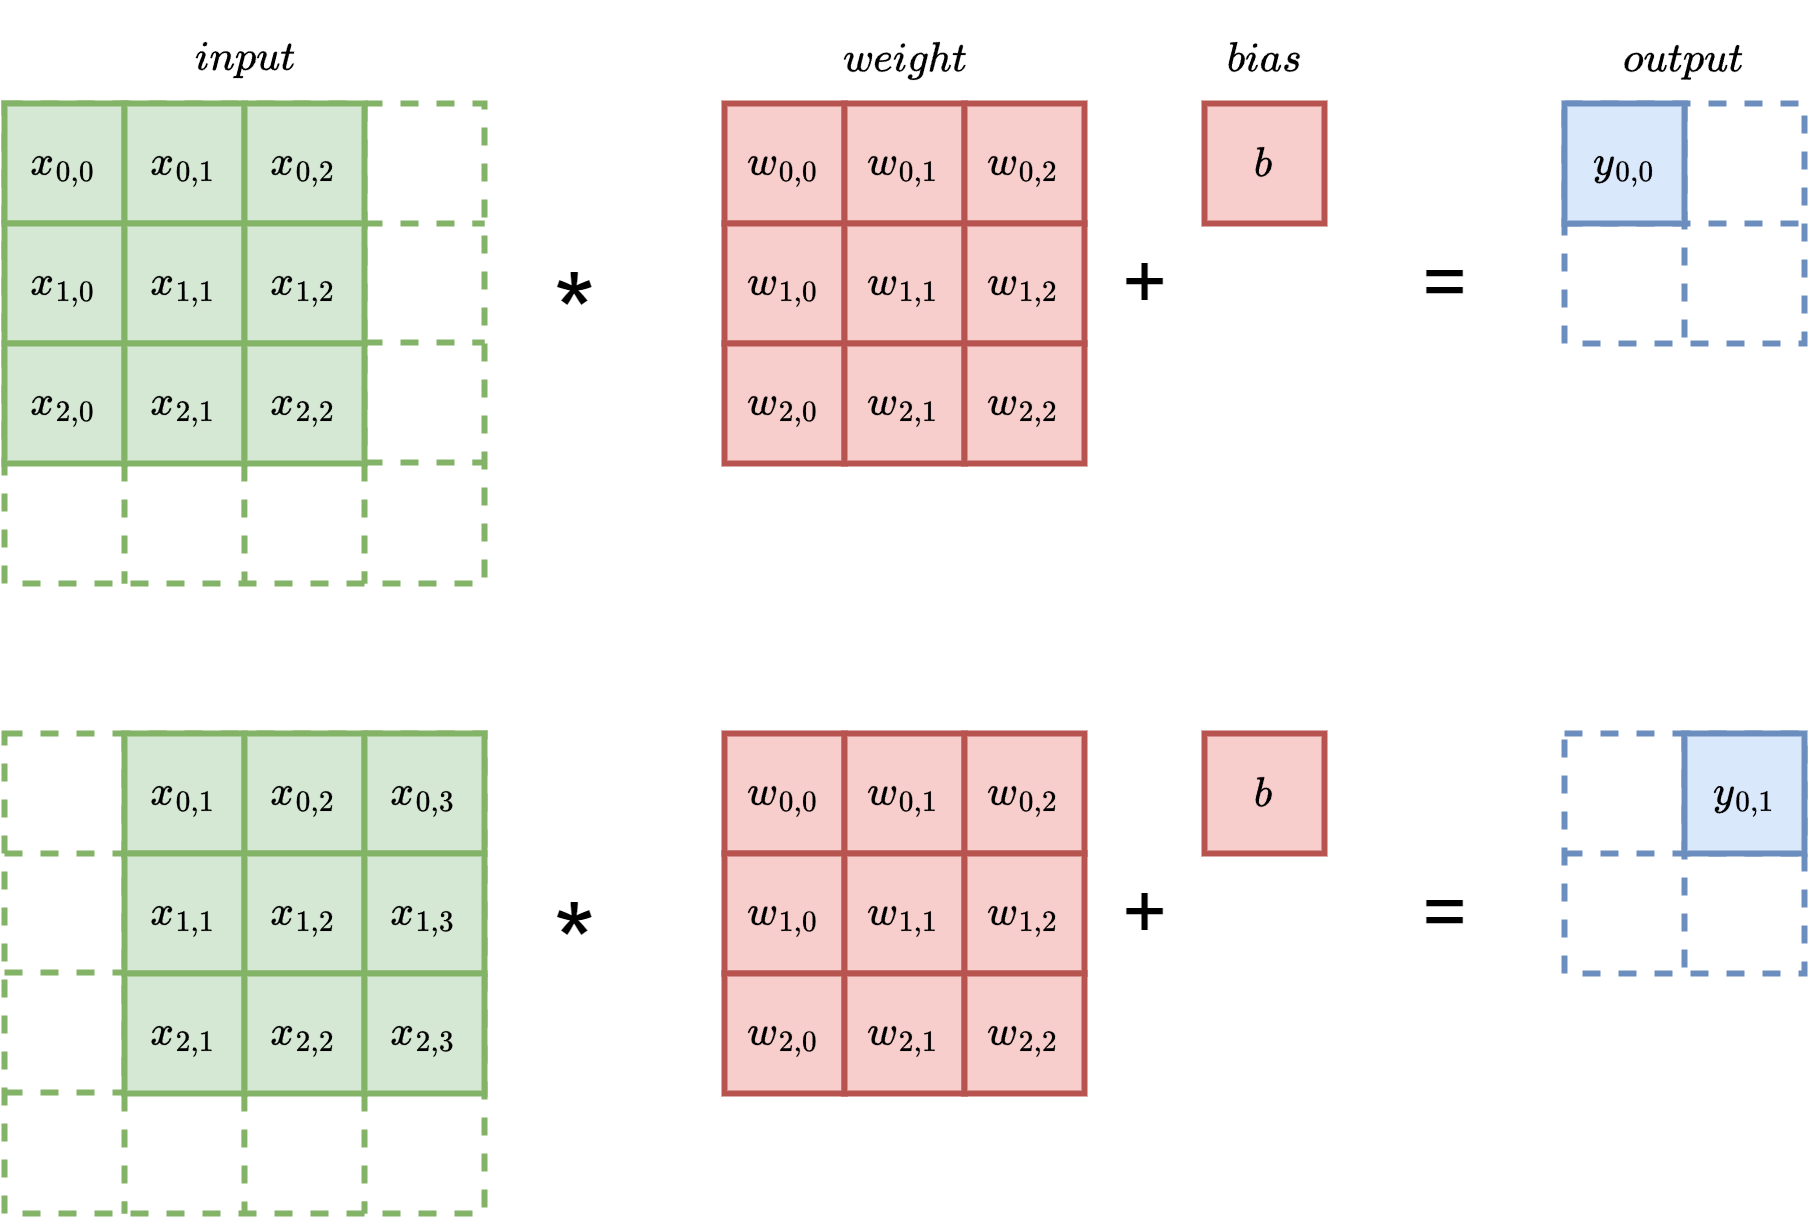
\includegraphics[width=0.6\linewidth]{src/conv.drawio (1).png}
    	\end{figure}
    	
    	\small
    	$y_{0, 0} = (x_{0, 0}*w_{0, 0} + x_{0, 1}*w_{0, 1} + x_{0, 2}*w_{0, 2} + x_{1, 0}*w_{1, 0} + x_{1, 1}*w_{1, 1} + x_{1, 2}*w_{1, 2} + x_{2, 0}*w_{2, 0} + x_{2, 1}*w_{2, 1} + x_{2, 2}*w_{2, 2}) + b$
    \end{frame}
    
    \subsection{Backpropagation}
    
    \begin{frame}
    	\frametitle{Backpropagation}
    	\begin{figure}
    		\centering
    		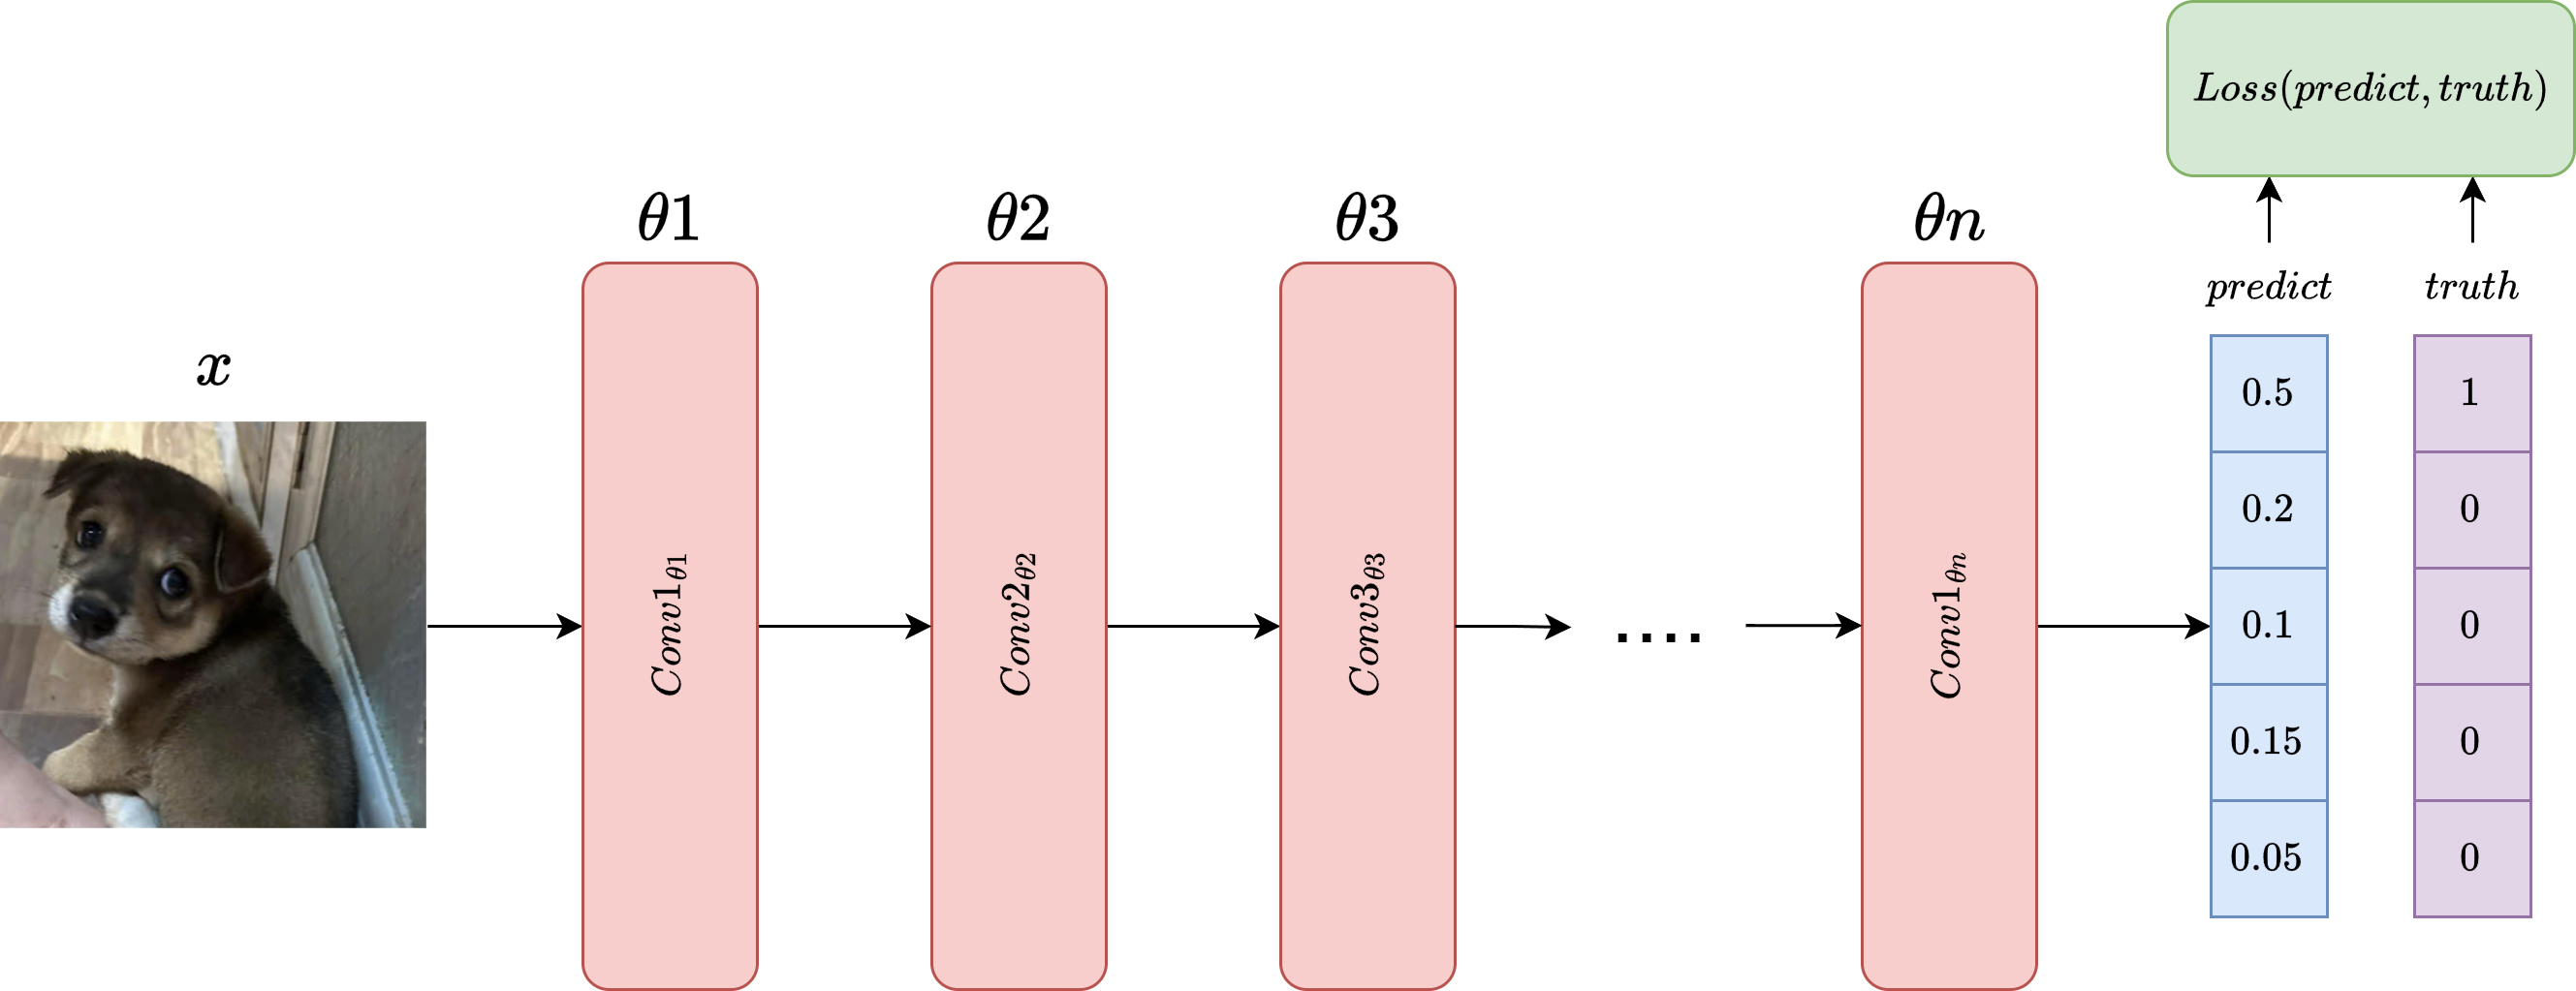
\includegraphics[width=0.8\linewidth]{src/backprop.drawio.png}
    	\end{figure}
    	
    	\justifying
    	Suppose we need to build a CNN for the image classification task. The input is an image \( x \), and there are \( n \) convolution layers \( f_\theta_i \), each parameterized by parameters \( \theta _i \). At this point, we can represent the output as:
    	
    	\[
    	\text{predict} = f_{\theta_n}(f_{\theta_{n-1}}(...(f_{\theta_1}(x))...)).
    	\]
    	
    \end{frame}
    
    \begin{frame}
    	\frametitle{Backpropagation}
    	\begin{figure}
    		\centering
    		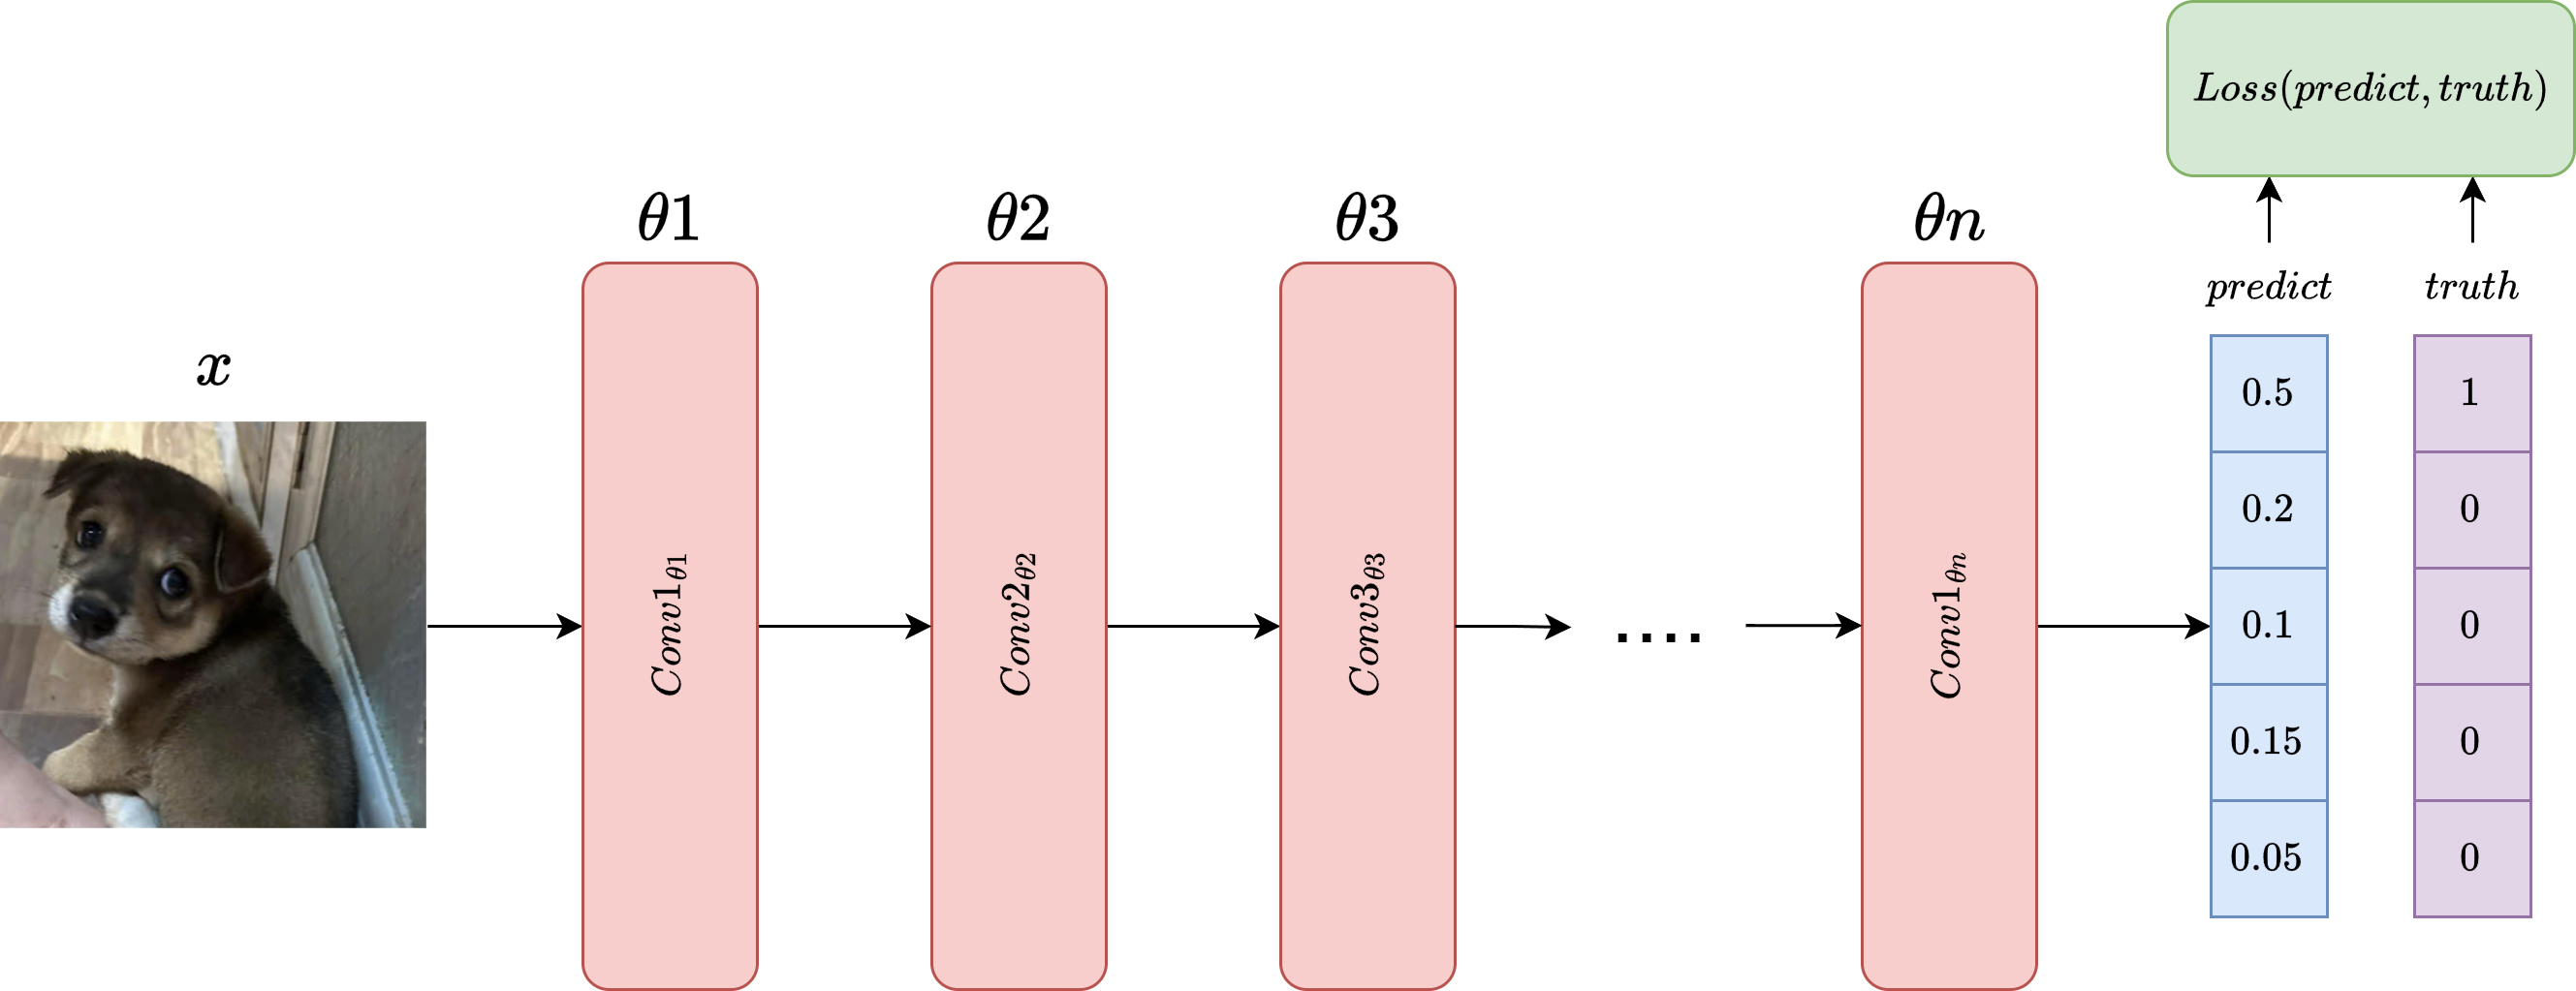
\includegraphics[width=0.8\linewidth]{src/backprop.drawio.png}
    	\end{figure}
    	
    	\justifying
    	Given a function \( \text{Loss}(\text{predict}, \text{truth}) \) that evaluates the fit between \( \text{predict} \) and \( \text{truth} \), the smaller the \( \text{Loss} \), the more accurate the model's predictions. We need to find the parameter set \( \theta = \{ \theta_1, \theta_2, \ldots, \theta_n \} \) that minimizes the \( \text{Loss} \)..
    	
    \end{frame}
    
    \begin{frame}
    	\frametitle{Backpropagation}   	
    	\justifying
    	At this point, you may realize that we only need to compute the generalized derivative and find the extrema of the \( \text{Loss} \) function with respect to \( \theta \). Unfortunately, this is practically infeasible due to the high dimensionality and complexity of the function. Although we cannot find the generalized derivative, for each input \( x \), we can compute the derivative of \( \text{Loss} \) with respect to \( \theta \) at \( x \). By moving in the direction opposite to the derivative, we will approach a local extremum of the \( \text{Loss} \).
    	
    	\[
    	\frac{\partial f(g(x))}{\partial x} = \frac{\partial f(g(x))}{\partial g(x)} \frac{\partial g(x)}{\partial x}
    	\]
    	
    	Since \( \text{predict} = f_{\theta_n}(f_{\theta_{n-1}}(...(f_{\theta_1}(x))...)) \) is a composite function, we can apply the chain rule above to calculate the derivative of \( \text{Loss} \) with respect to each \( \theta_i \) one by one. The first derivative is taken at the output and then traced back to the input, which is why it is called backpropagation.
    \end{frame}
    
    \subsection{Derivative of Weight}
    
    \begin{frame}
    	\frametitle{Derivative of Weight}
    	\justifying
   
    	\begin{figure}
    		\centering
    		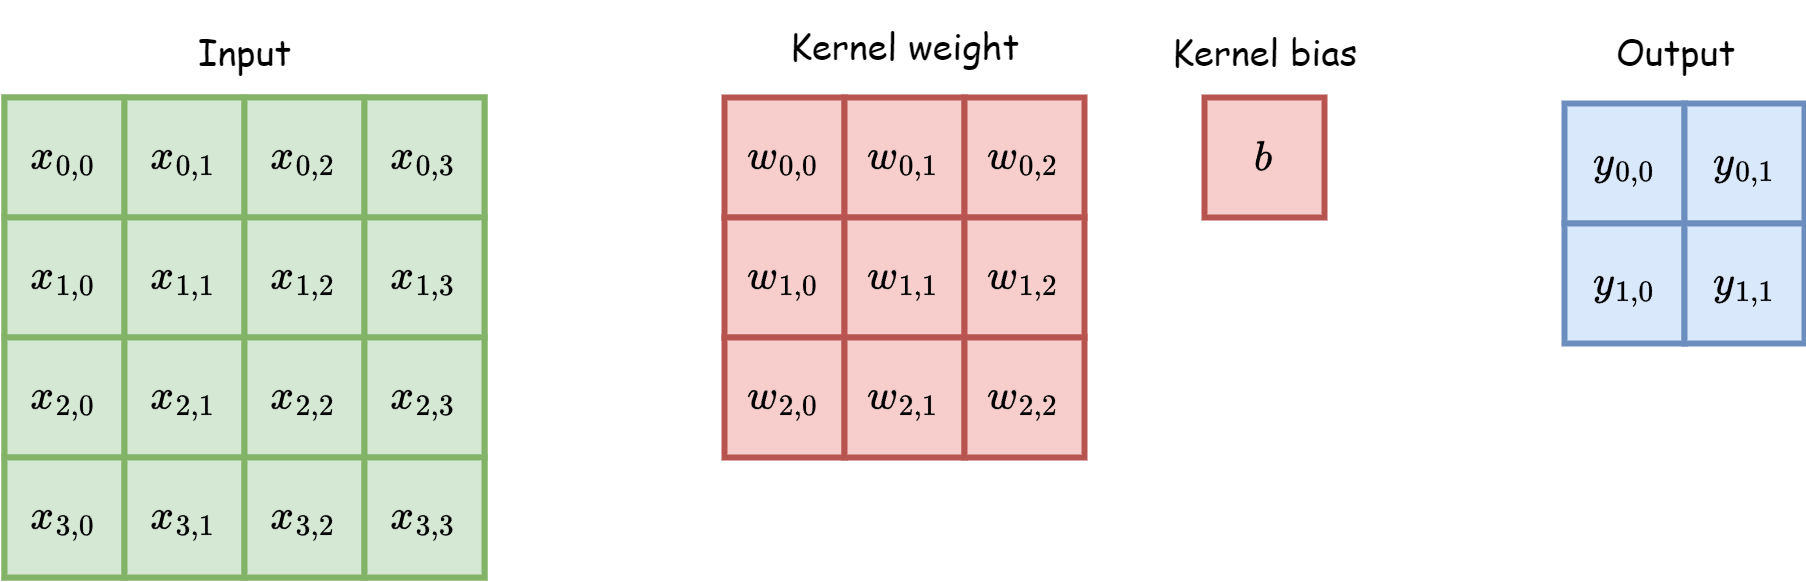
\includegraphics[width=0.8\linewidth]{src/conv.drawio (2).png}
    	\end{figure}
    	
    	\begin{align*}
    		\frac{\partial Loss(x)}{\partial weight} = \frac{\partial Loss(x)}{\partial output} \frac{\partial output}{\partial weight}
    	\end{align*}
    \end{frame}
    
    \begin{frame}
    	\frametitle{Derivative of Weight}
    	\begin{figure}
    		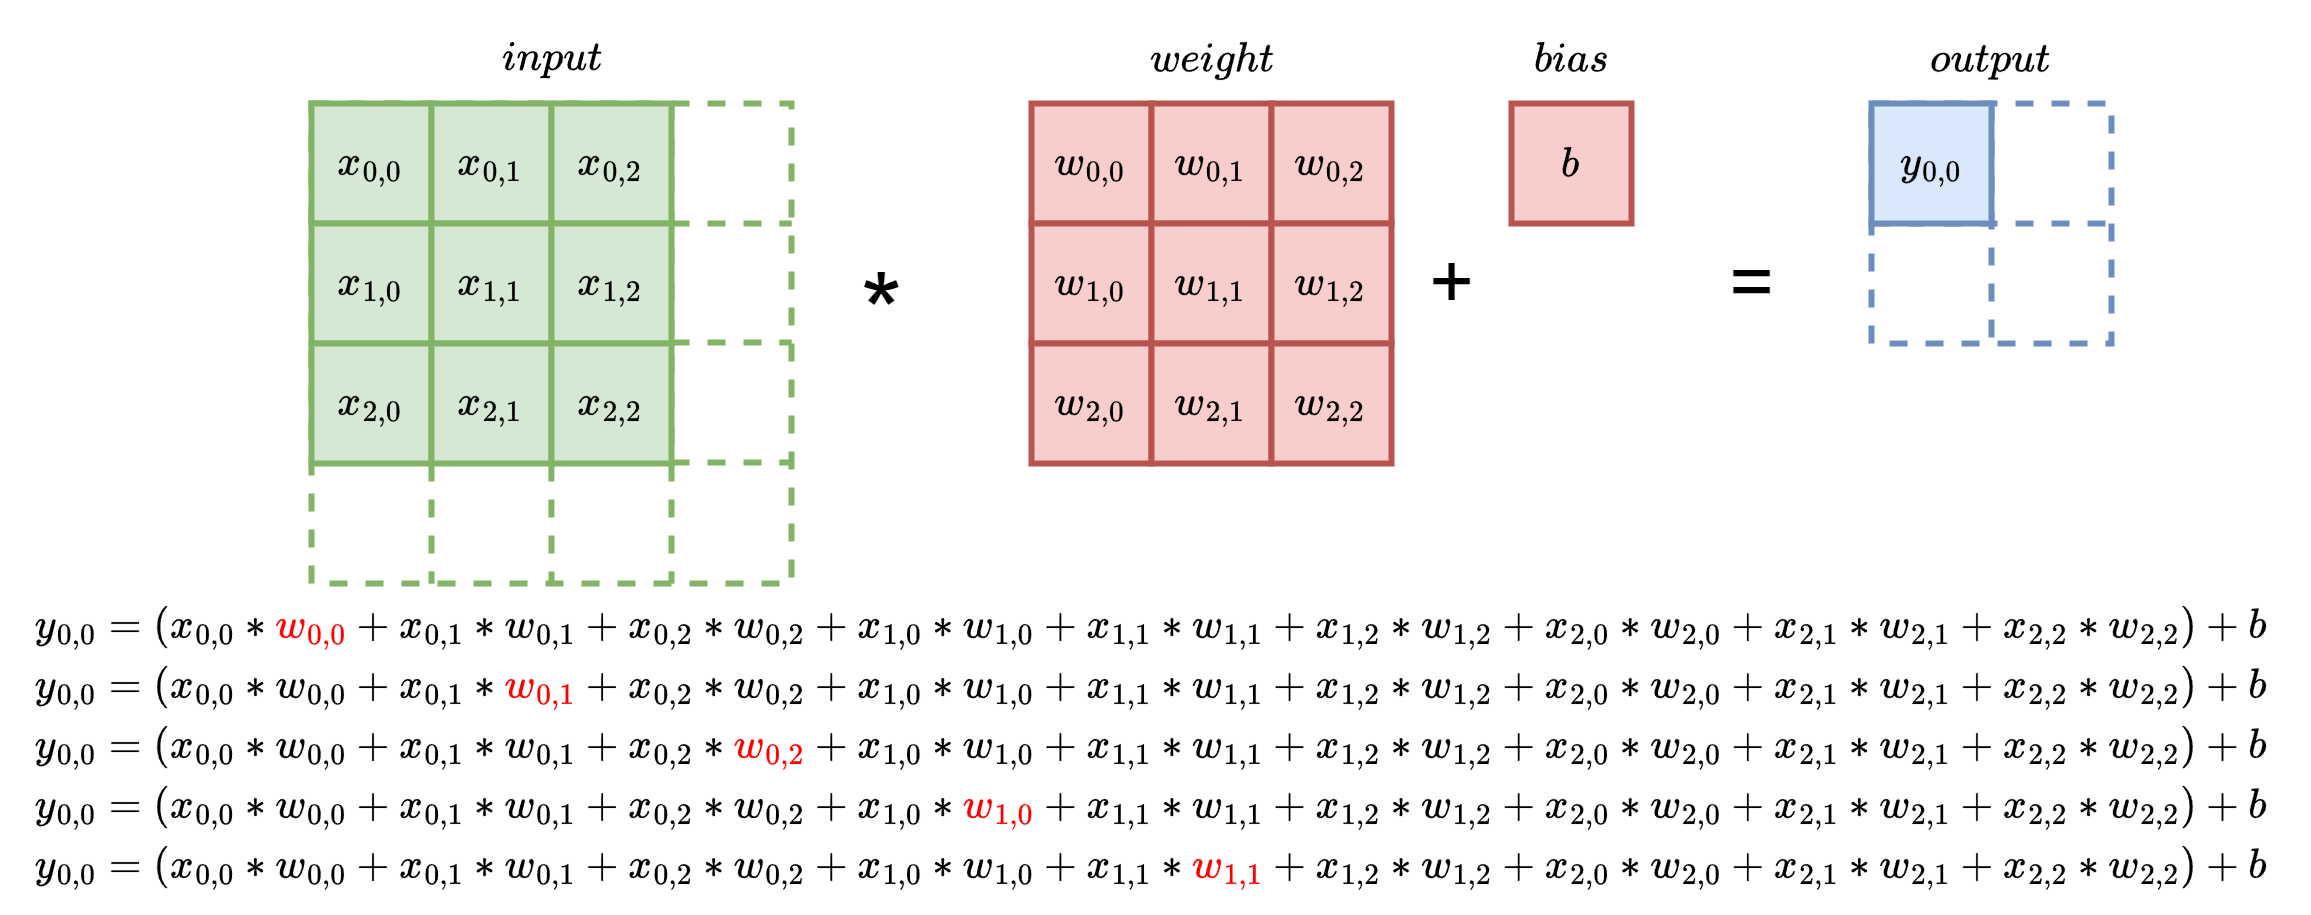
\includegraphics[width=1.\linewidth]{src/backprop_weight.drawio.png}
    	\end{figure}
    \end{frame}
    
    \begin{frame}
    	\frametitle{Derivative of Weight}
    	
    	% TODO: \usepackage{graphicx} required
    	\begin{figure}
    		\centering
    		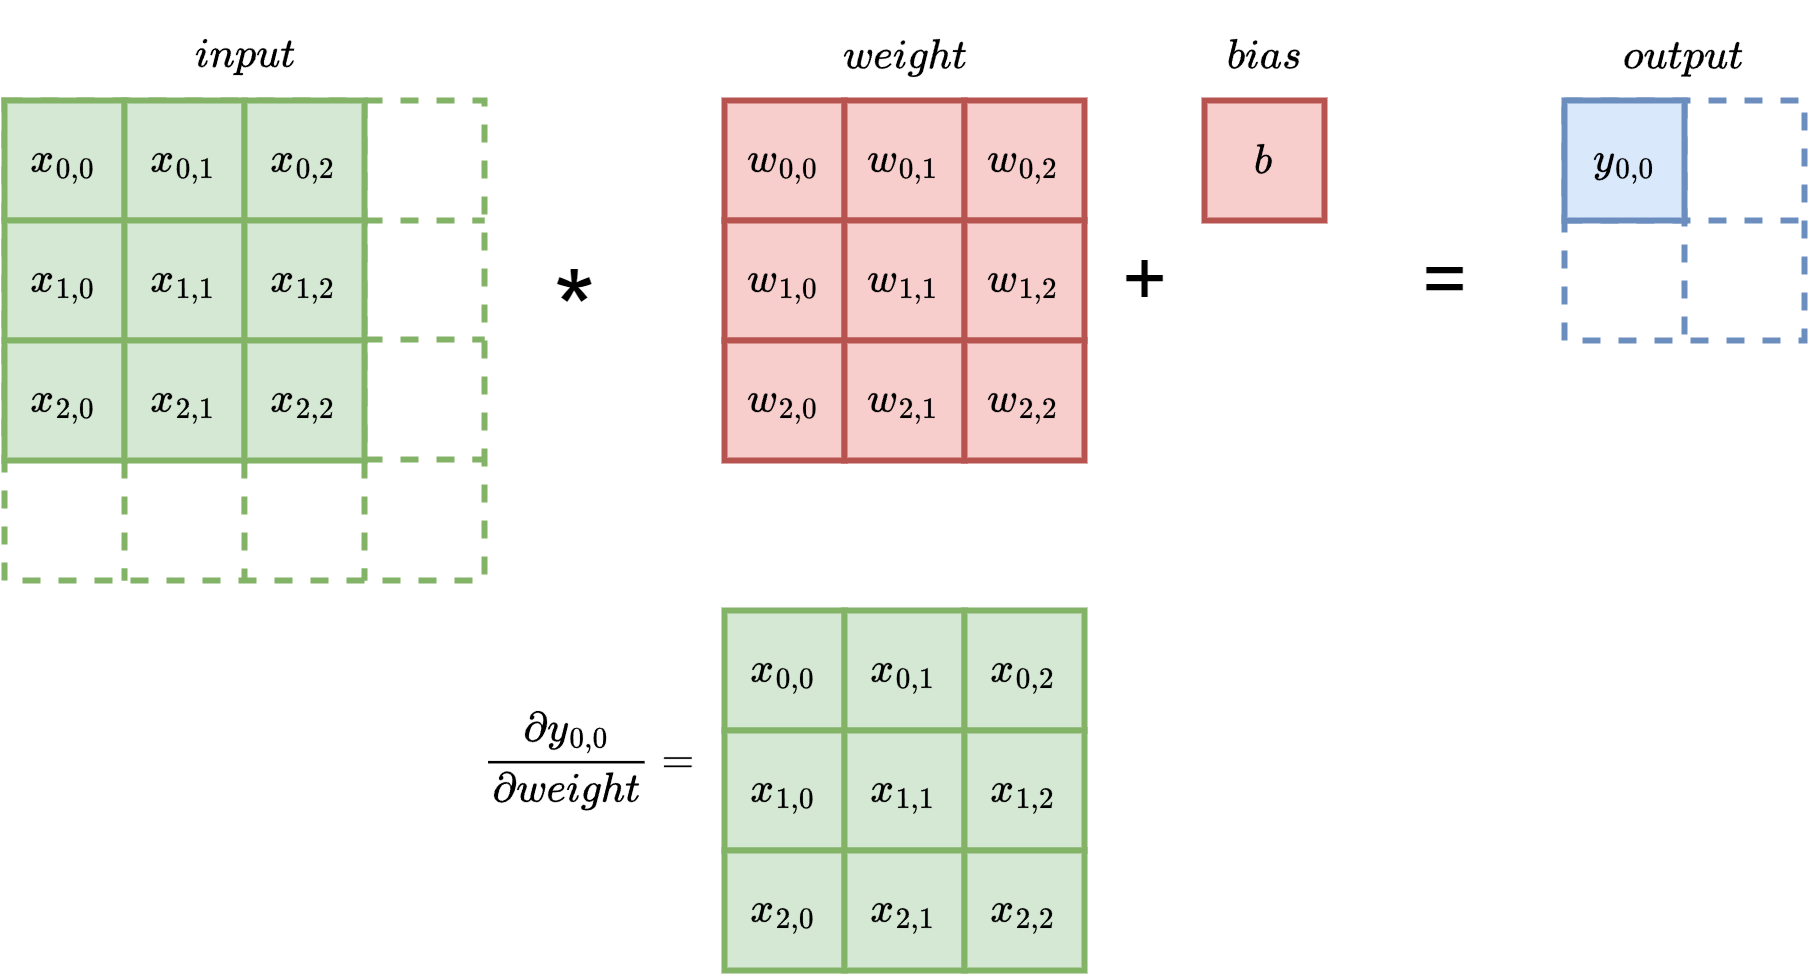
\includegraphics[width=0.9\linewidth]{src/dweight.drawio}
    		\label{fig:dweight}
    	\end{figure}
    \end{frame}
    
    
    \begin{frame}
    	\frametitle{Derivative of Weight}
    	
% TODO: \usepackage{graphicx} required
\begin{figure}
	\centering
	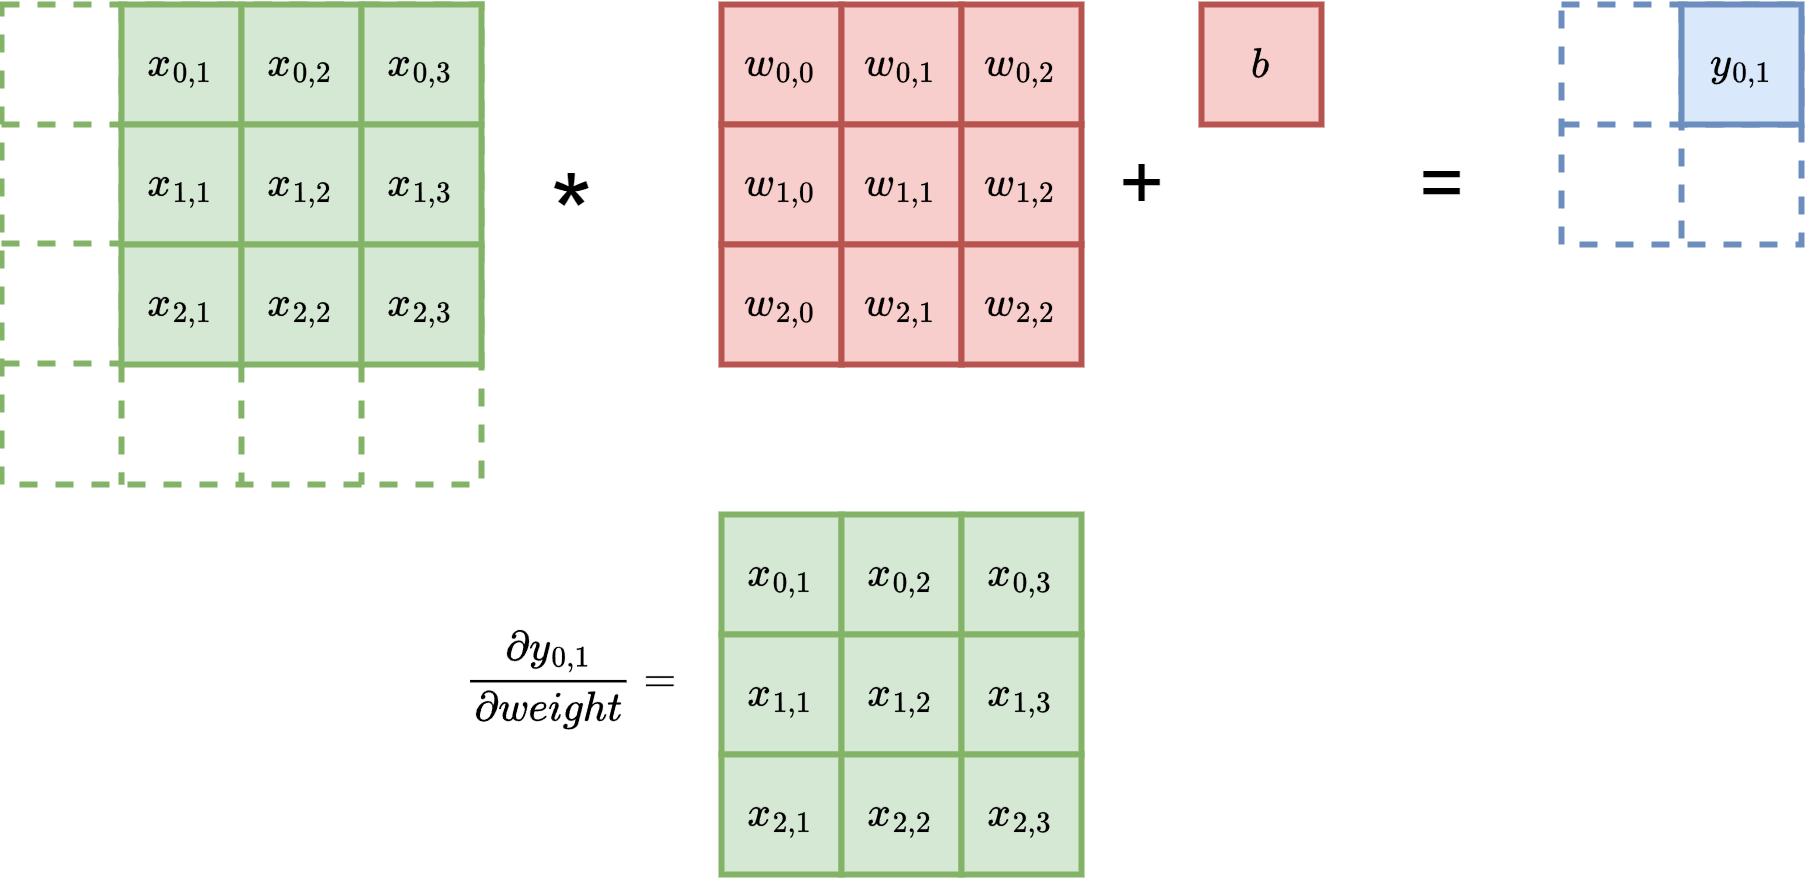
\includegraphics[width=1.0\linewidth]{src/weight_grad.drawio}
\end{figure}
    \end{frame}
    
    \begin{frame}
    	\frametitle{Derivative of Weight}
    	
% TODO: \usepackage{graphicx} required
\begin{figure}
	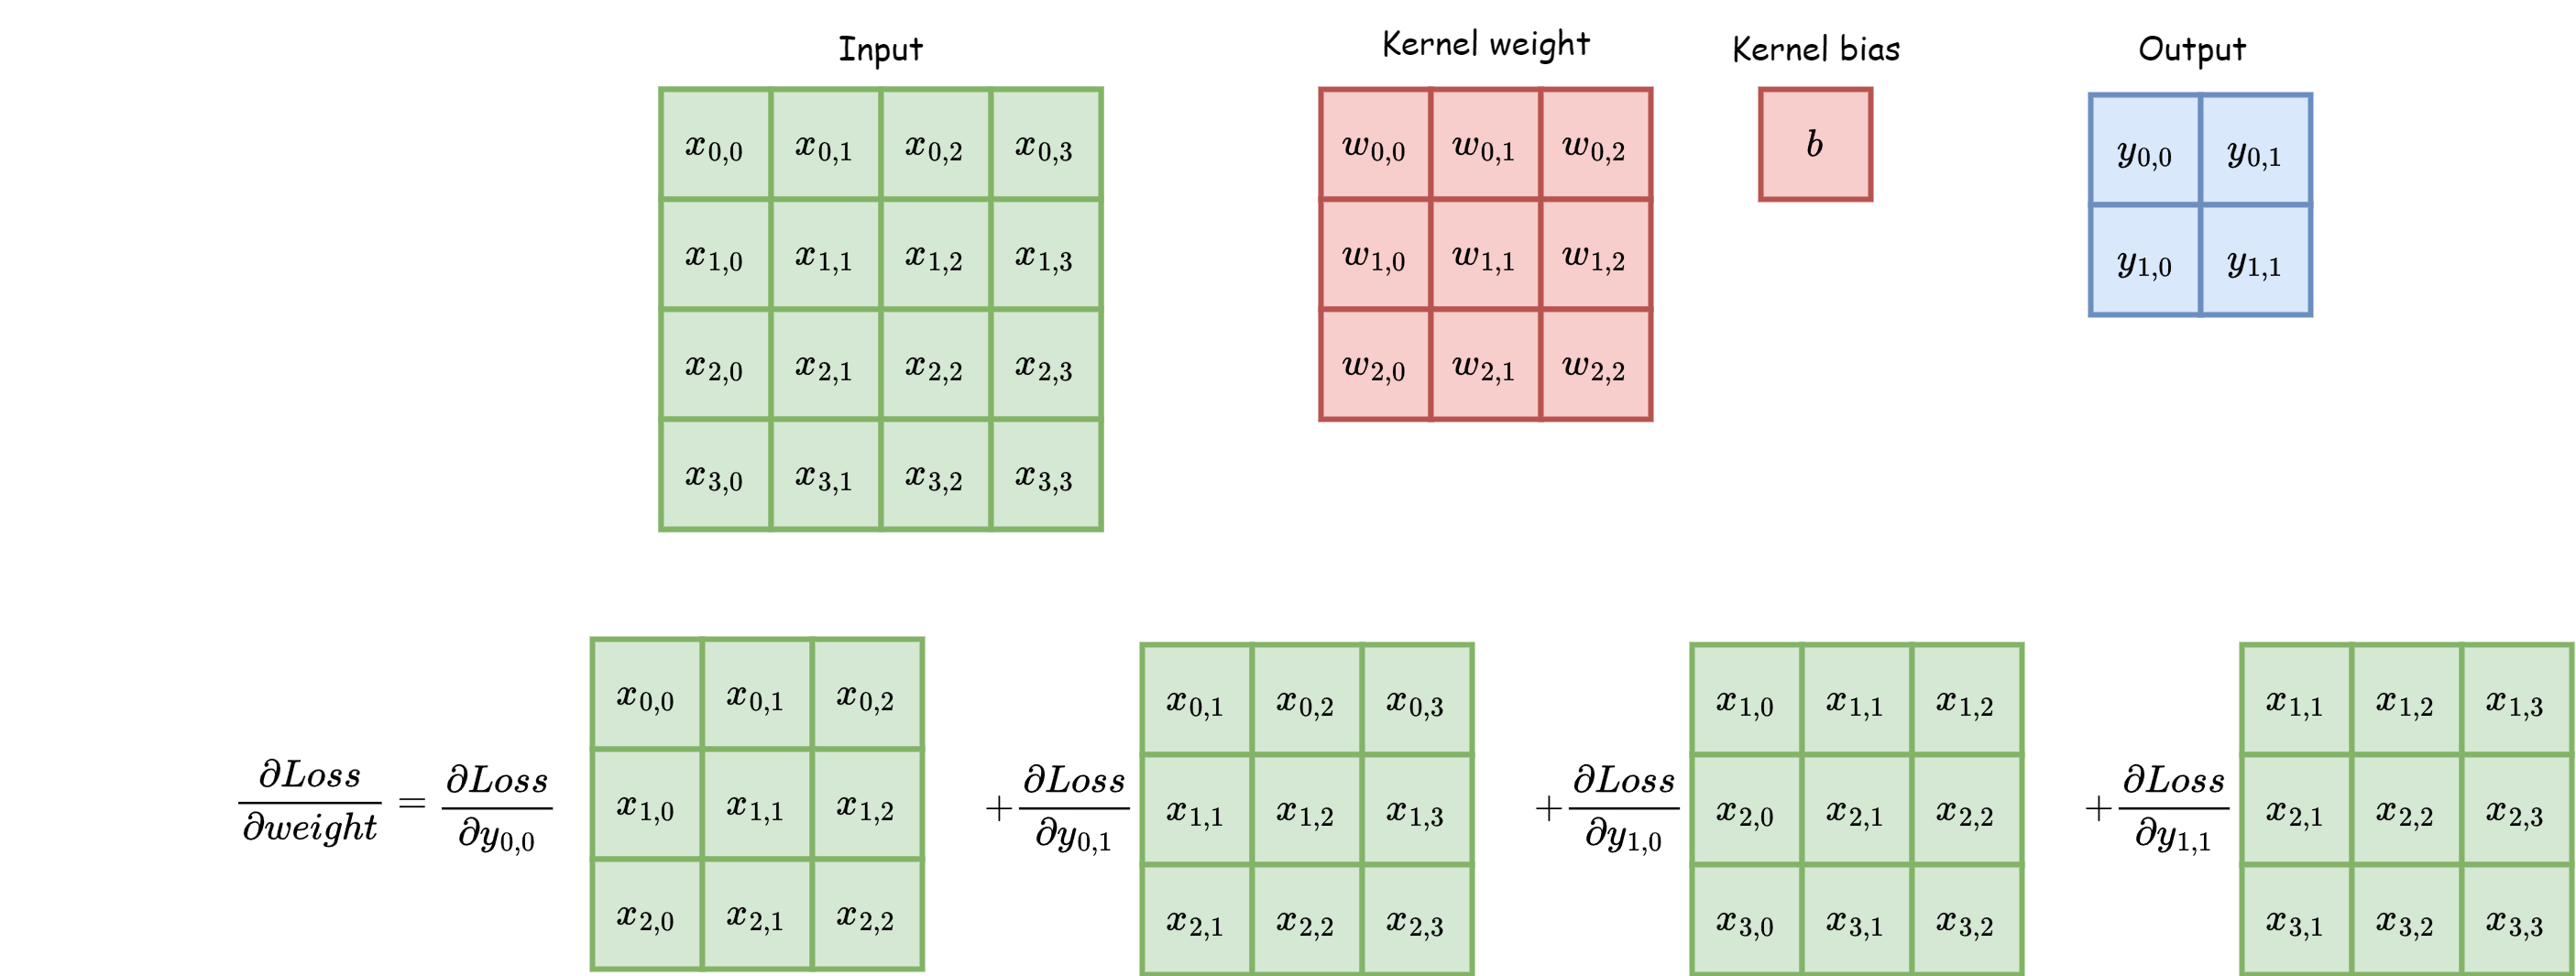
\includegraphics[width=1.\linewidth]{src/derivative.drawio}
\end{figure}
    \end{frame}
    
    \subsection{Derivative of Bias}
    
    
    \begin{frame}
    	\frametitle{Derivative of Convolution}
    	\begin{figure}
    		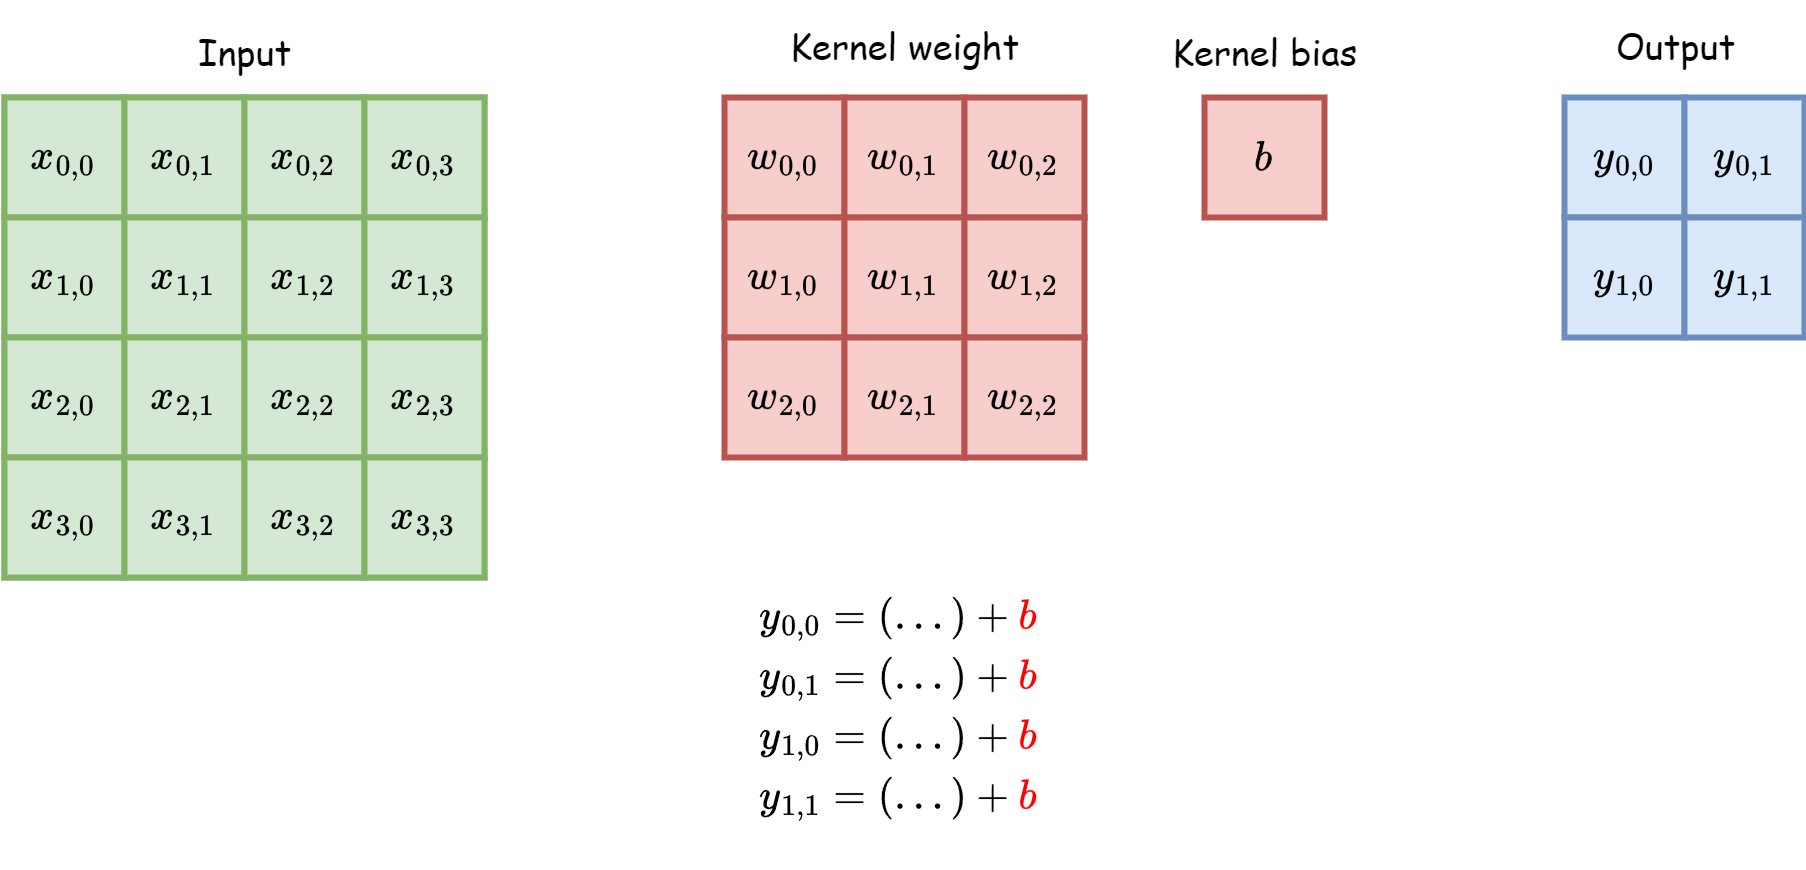
\includegraphics[width=1.\linewidth]{src/bias_grad.drawio (1)}
    	\end{figure}
    \end{frame}
    
    \begin{frame}
    	\frametitle{Derivative of bias}
    	
    	% TODO: \usepackage{graphicx} required
    	\begin{figure}
    		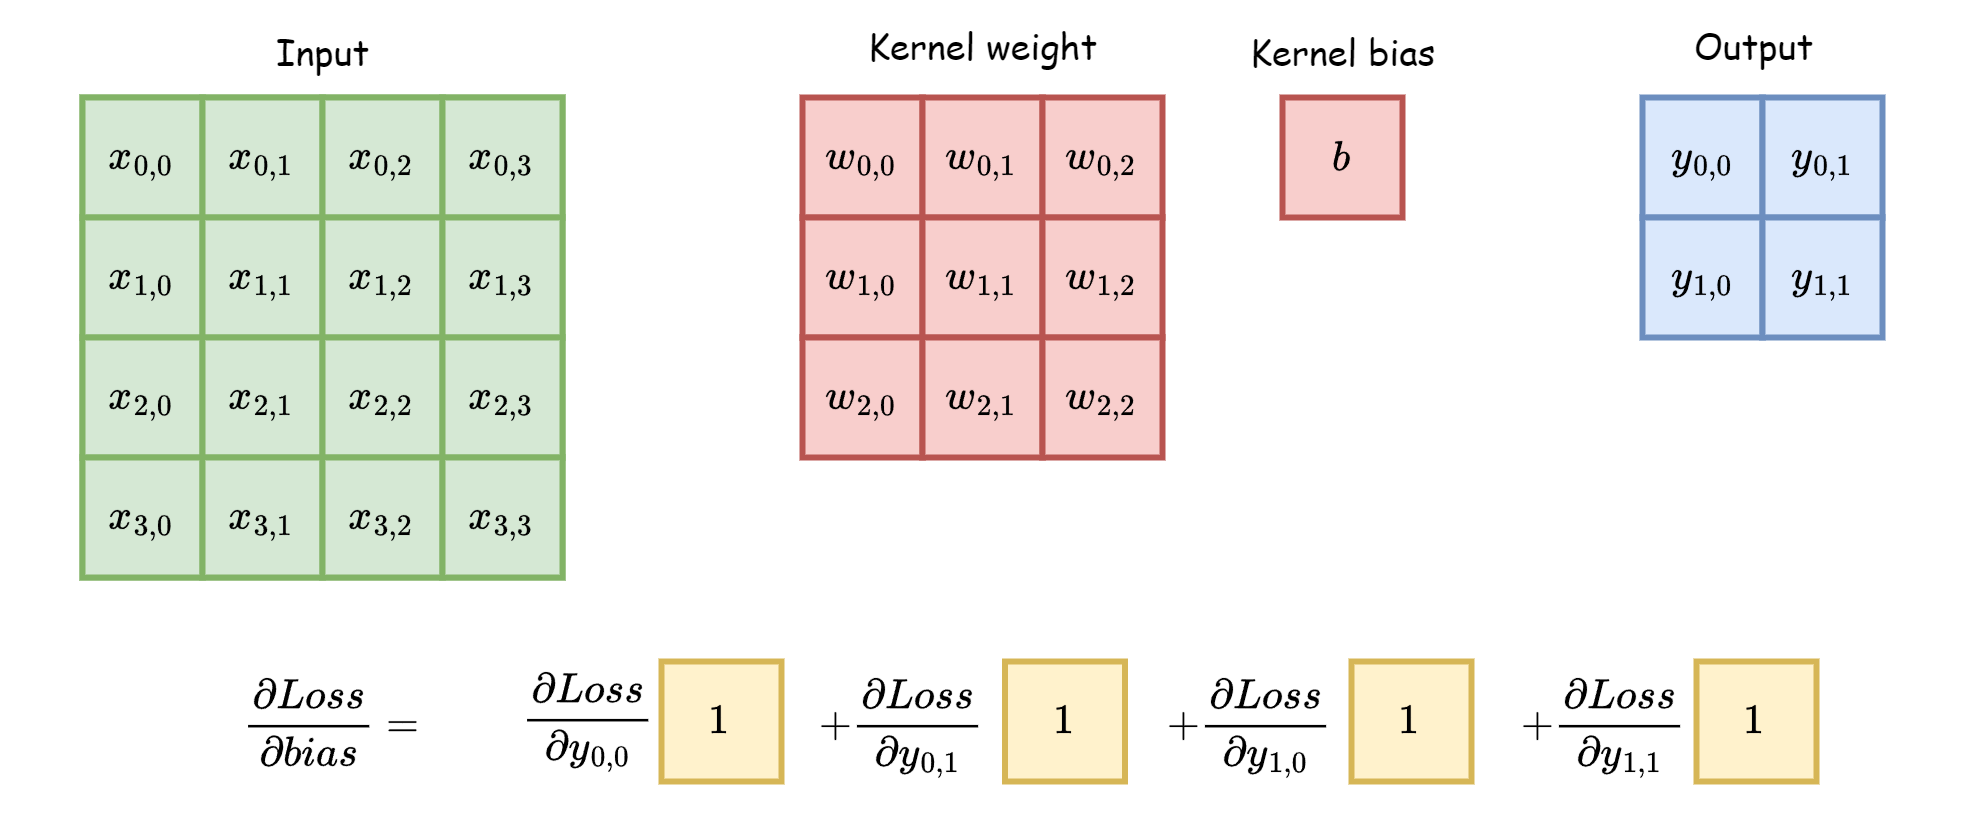
\includegraphics[width=1.\linewidth]{src/bias_grad.drawio}
    	\end{figure}
    \end{frame}
    
    \subsection{Derivative of Input}
    
    \begin{frame}
    	\frametitle{Derivative of Input}
		\begin{figure}
			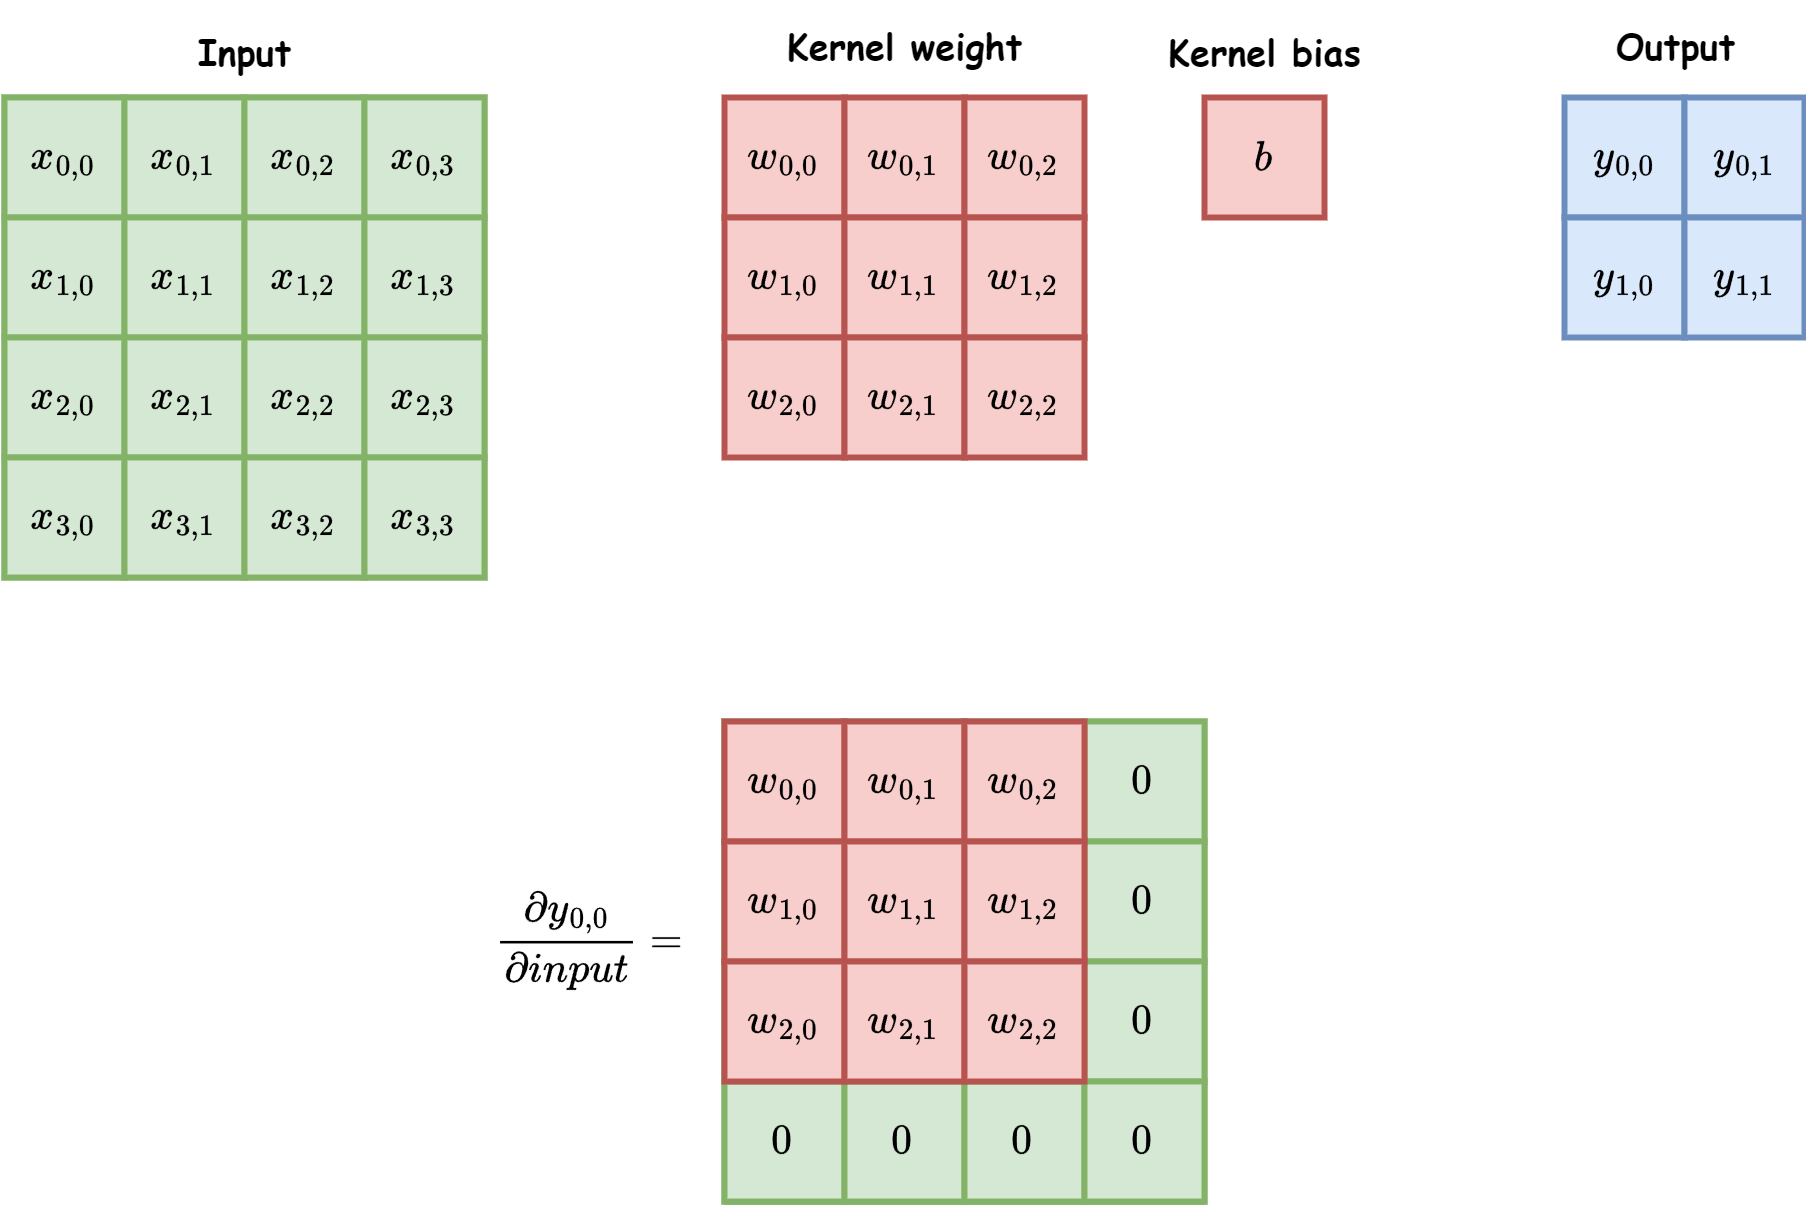
\includegraphics[width=0.7\linewidth]{src/input_grad.drawio}
		\end{figure}
    \end{frame}
    
    \begin{frame}
    	\frametitle{Derivative of Input}
		\begin{figure}
			\includegraphics[width=0.7\linewidth]{"src/input_grad.drawio (1)"}
		\end{figure}
    \end{frame}
    
    \begin{frame}
    	\frametitle{Derivative of Input}
		\begin{figure}
			\includegraphics[width=1.\linewidth]{"src/input_grad.drawio (2)"}
		\end{figure}
    \end{frame}
    
    \subsection{Derivative of Padding}
    \begin{frame}
	\frametitle{Derivative of Padding}
    	\begin{figure}
    		\includegraphics[width=0.8\linewidth]{"src/conv2.drawio"}
    	\end{figure}
    \end{frame}
	
	\begin{frame}
		\frametitle{Derivative of Padding}
		\begin{figure}
			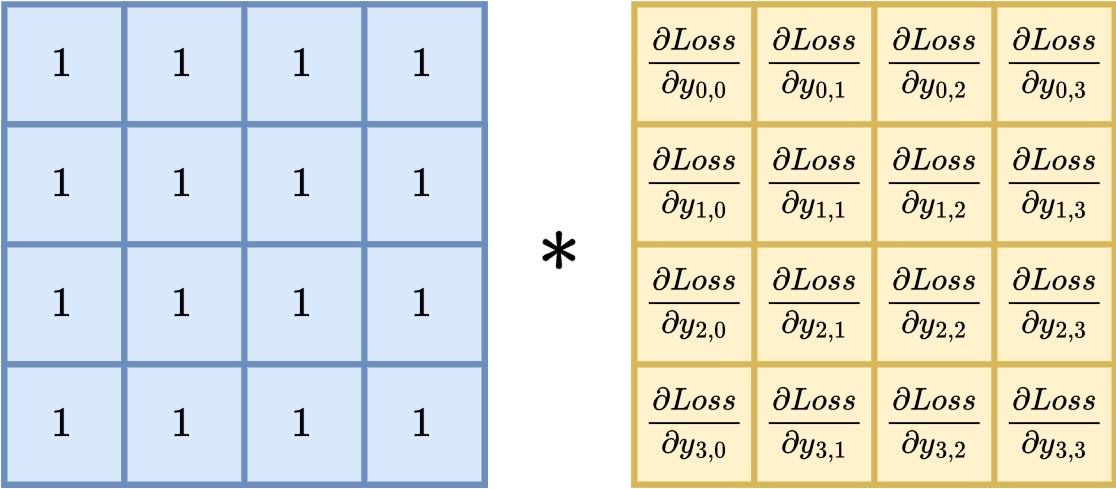
\includegraphics[width=0.8\linewidth]{"src/conv.drawio3.png"}
		\end{figure}
	\end{frame}
    
    \subsection{Derivative of MaxPool}
    \begin{frame}
    	\frametitle{Derivative of MaxPool}
    	\begin{figure}
    		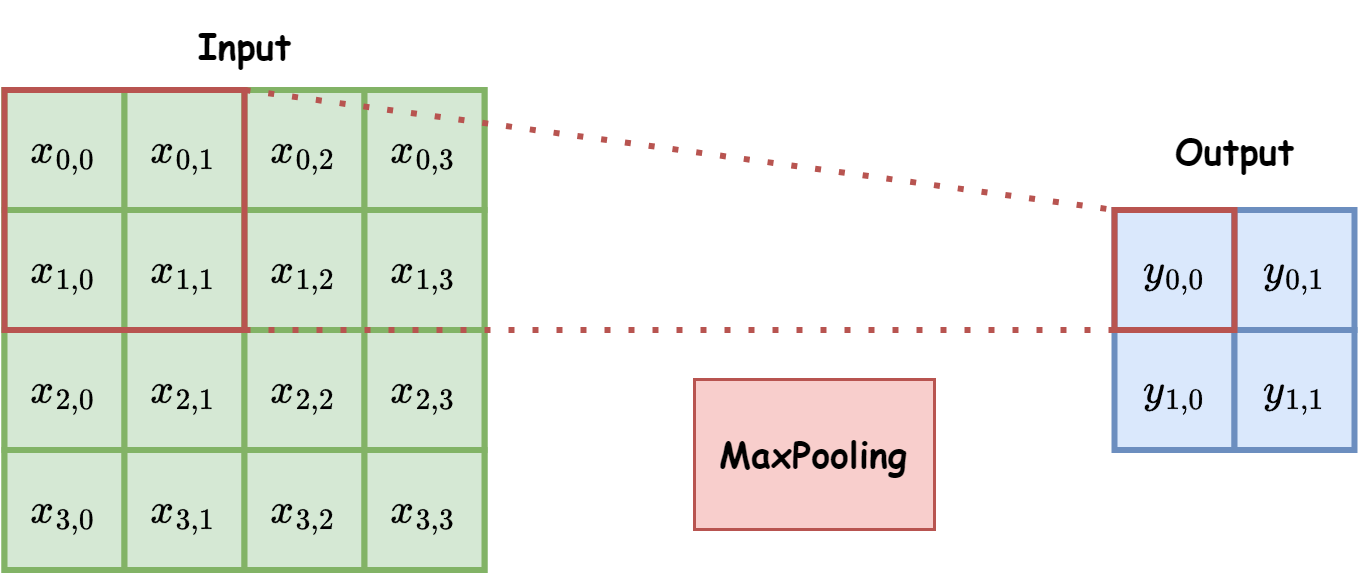
\includegraphics[width=0.8\linewidth]{"src/conv.drawio (3).png"}
    	\end{figure}
    \end{frame} 
    
    \begin{frame}
    	\frametitle{Derivative of MaxPool}
    	\begin{figure}
    		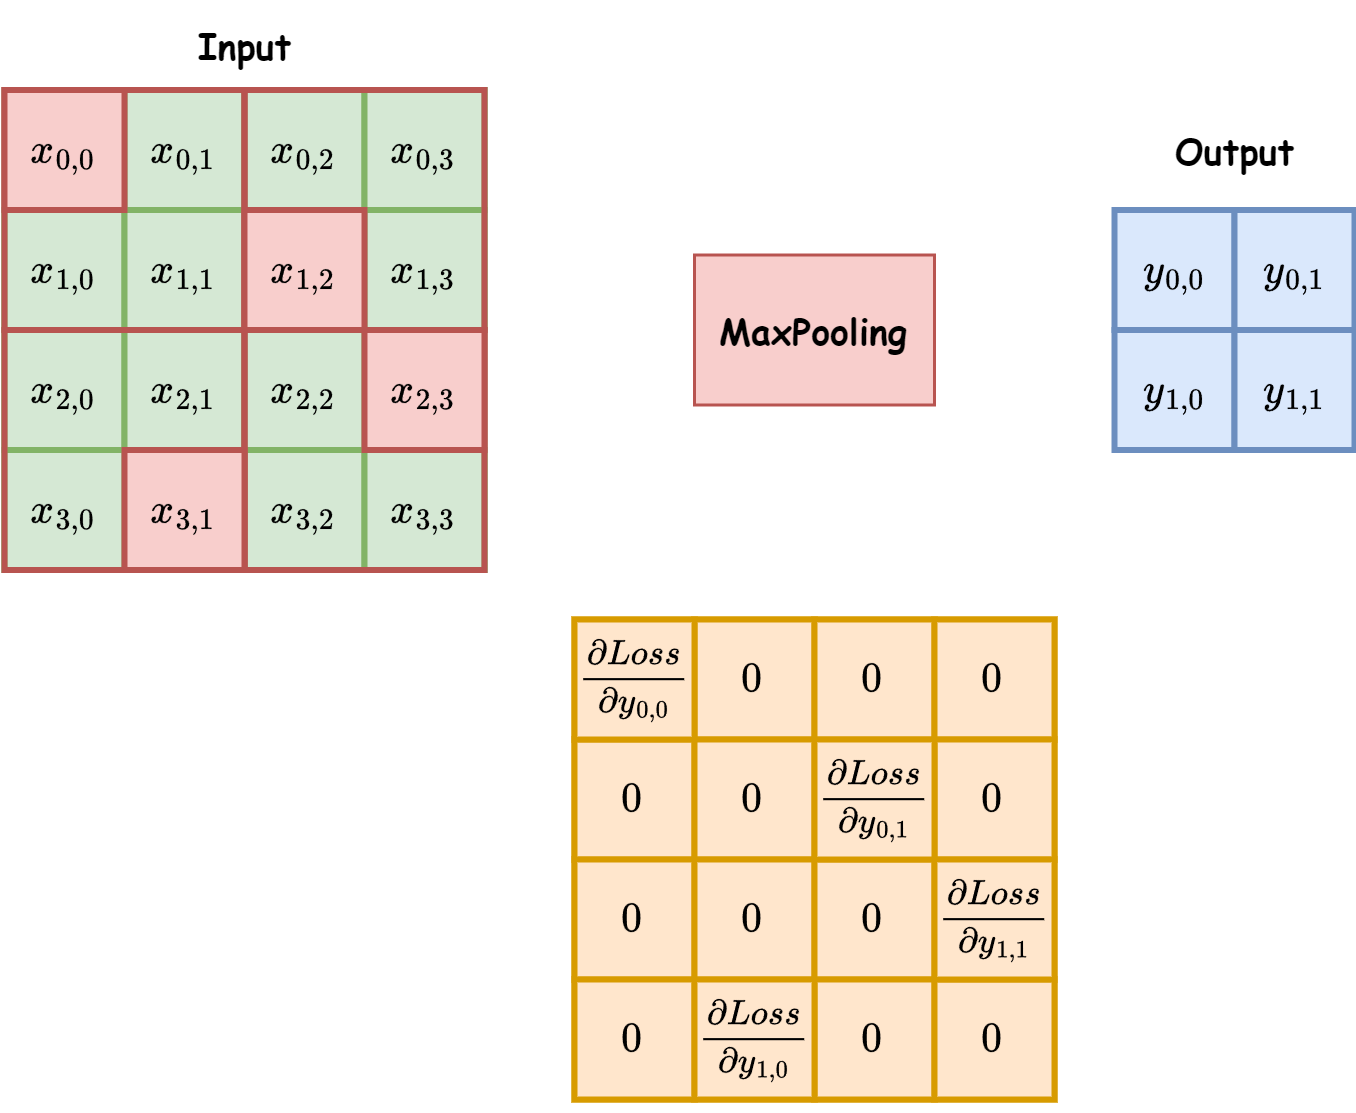
\includegraphics[width=0.6\linewidth]{"src/conv.drawio (4).png"}
    	\end{figure}
    \end{frame} 
  
    \subsection{Derivative of ReLU}  
    \begin{frame}
    	\frametitle{Derivative of ReLU}
    	\begin{figure}
    		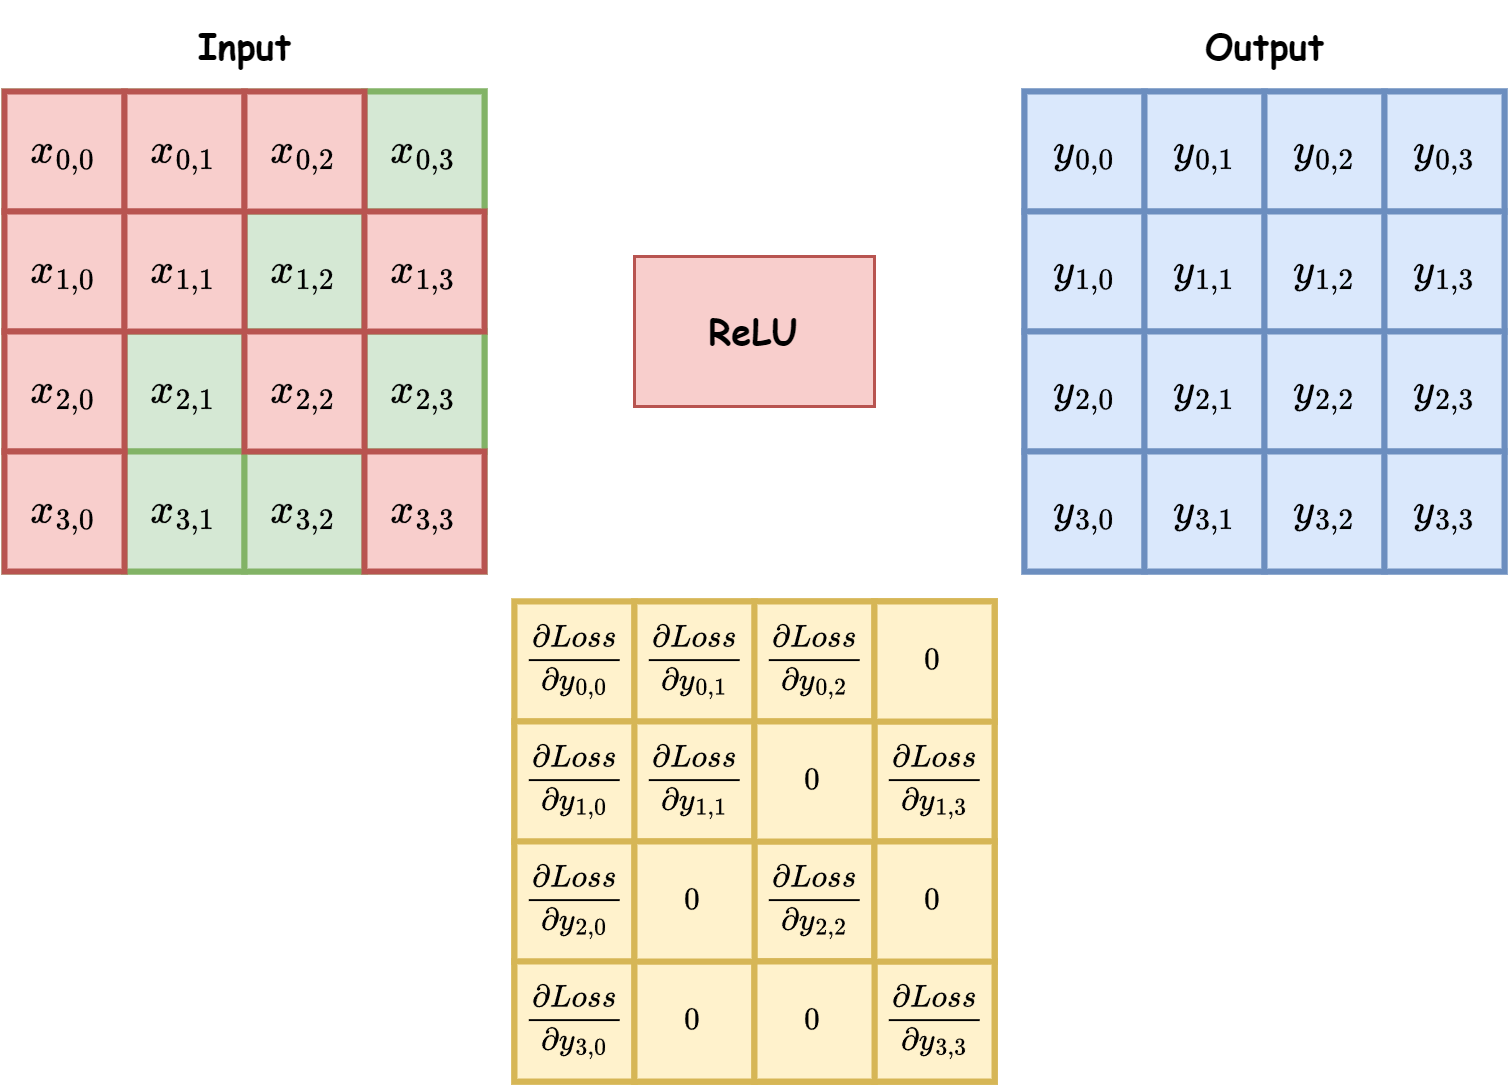
\includegraphics[width=0.6\linewidth]{"src/conv.drawio (5).png"}
    	\end{figure}
    \end{frame} 
    
    \subsection{Derivative of Cross Entropy}
    
    \begin{frame}
    	\frametitle{Derivative of Cross Entropy}
    	\justifying
    	The problem we set out to solve is image classification, where the output \( \text{predict} \in \mathbb{R}^N \) with \( \text{predict}[i] \) being the prediction for class \( i \), and the label \( \text{truth} \in \mathbb{R}^n \) (abbreviated as \( t \)) is a one-hot vector. We have the Softmax function:
    	
    	\[
    	p_i = \frac{e^{\text{predict}[i]}}{\sum_{j=1}^{N} e^{\text{predict}[j]}} 
    	\]
    	
    	The cross-entropy loss function is defined as (using natural logarithm):
    	
    	\[
    	\text{Loss} = -\sum_{i=1}^N t[i] \log(p[i])
    	\]
    \end{frame}
    
    \begin{frame}
    	\frametitle{Derivative of Cross Entropy}
    	However, the vector \( t \) is one-hot, with only one value being \( 1 \) and the rest being \( 0 \). Let \( k \) be the index where \( t[k] = 1 \). Thus, the loss function can be simplified to:
    	
    	\[
    	\text{Loss} = -\log(p[k])
    	\]
    	
    	Let’s recall some derivatives of composite functions \( u \) and \( v \):
    	
 
    	\begin{align*}
    		(\log(u))' &= \frac{u'}{u} \\
    		\left(\frac{1}{u}\right)' &= \frac{-u'}{u^2} \\
    		(uv)' &= u'v + uv'
    	\end{align*}
    \end{frame}
    
    \begin{frame}
    	\frametitle{Derivative of Cross Entropy}
    	We need to calculate \( \frac{\partial \text{Loss}}{\partial \text{predict}} \) (from now on, we will refer to \( \text{predict} \) as \( x \)):
    	For $x[i]$ where $i=k$:
    	\begin{align*}
    		\frac{\partial Loss}{\partial x[i]} &= -\frac{\partial log(p[k])}{\partial x[i]}\\
    		&= -\frac{1}{p[k]} \frac{\partial p[k]}{\partial x[i]}\\
    		&= -\frac{1}{p[k]} (\frac{e^{x[k]}}{\sum_{j=1}^N e^{x[j]}} - (\frac{e^{x[k]}}{\sum_{j=1}^N e^{x[j]}})^2)\\
    		&= -\frac{1}{p[k]} (p[k] - p[k]^2)\\
    		&= -(1 - p[k])\\
    		&= p[k] - 1
    	\end{align*}
    \end{frame}
    
    \begin{frame}
    	\frametitle{Derivative of Cross Entropy}
    	For $x[i]$ where $i\neq k$:
    	\begin{align*}
    		\frac{\partial Loss}{\partial x[i]} &= -\frac{\partial log(p[k])}{\partial x[i]}\\
    		&= -\frac{1}{p[k]} \frac{\partial p[k]}{\partial x[i]}\\
    		&= -\frac{1}{p[k]} (-\frac{e^{x[i]}e^{x[k]}}{(\sum_{j=1}^N e^{x[j]})^2})\\
    		&= \frac{1}{p[k]}(p[k]p[i])\\
    		&= p[i]
    	\end{align*}
    \end{frame}
    
    \section{Experiment}
    \subsection{Setting}
    
    \begin{frame}[fragile]
    	\frametitle{Model}
    	\justifying
    	Based on the above theory, I built a model using Conv2D, ReLU, Softmax, and the Cross Entropy loss function entirely with NumPy (not using PyTorch's autograd in the model, only for the purpose of checking consistency of results) and manually computed derivatives. The code is attached in the document. The model consists of 6 Conv layers:
\begin{multicols}{2}
	\small
	\begin{lstlisting}[language=Python]
		def __init__(self, input_dim, eta=1e-4):
		self.input_dim = input_dim
		self.eta = eta
		
		self.conv1    = Conv2D(1, 16, 3)
		self.padding1 = Padding(1)
	\end{lstlisting}
	\begin{lstlisting}[language=Python]
		self.relu1    = ReLU()
		
		self.conv2    = Conv2D(16, 32, 3)
		self.padding2 = Padding(1)
		self.relu2    = ReLU()
		self.maxpool  = MaxPool(2)
		
		self.conv3    = Conv2D(32, 64, 3)
		self.relu3    = ReLU()
	\end{lstlisting}
	\begin{lstlisting}[language=Python]
		self.conv4    = Conv2D(64, 64, 3)
		self.relu4    = ReLU()
		
		self.flatten  = Flatten()
		
		self.conv5    = Conv2D(64*10*10, 10, 1)
		
		self.loss  = Loss()
	\end{lstlisting}
\end{multicols}
    \end{frame}
    
        \begin{frame}{MNIST}{\thesection \, \secname}
    	MNIST is a dataset for handwritten digit classification consisting of 60,000 training images and 10,000 test images (28x28 pixels).
    	
    	% TODO: \usepackage{graphicx} required
    	\begin{figure}
    		\centering
    		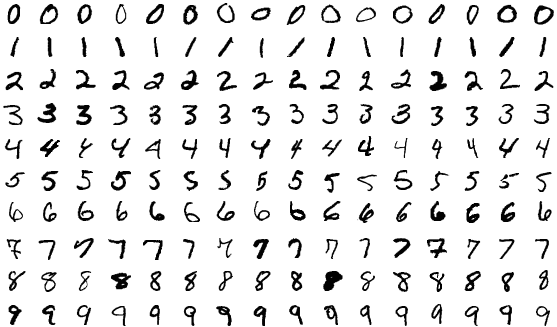
\includegraphics[width=0.6\linewidth]{src/MnistExamplesModified}
    	\end{figure}
    \end{frame}
    
    \subsection{Kết quả trực quan}
    \begin{frame}
    	\frametitle{Visualize}
    	Visualize time!
    \end{frame}

    \QApage

\end{document}
